\documentclass[journal,article,submit,pdftex,moreauthors]{Definitions/mdpi} 

\Title{Aplikasi MediSmart untuk Mendeteksi Penyakit Kulit}

\TitleCitation{Title}

\newcommand{\orcidauthorA}{0000-0000-0000-000X}

% Preamble untuk menambahkan paket atau pengaturan tambahan
\usepackage{pgfplots} % Paket untuk membuat grafik
\usepackage{graphicx}
\usepackage{caption}
\pgfplotsset{compat=1.18} % Pengaturan versi pgfplots yang digunakan
\renewcommand{\figurename}{Gambar}

\Author{Aan Syawaluddin Adi Putra $^{1}, Elva Aprili Timang $^{2}$, Khaerurrozikin $^{3}$, Zabryna Andiny $^{4}$, Alqadri $^{5}$, dan Sakinah Nurusyifa$^{6}$}


\AuthorNames{Firstname Lastname, Firstname Lastname and Firstname Lastname}

\AuthorCitation{Lastname, F.; Lastname, F.; Lastname, F.}

\address{%
$^{1}$ \quad Universitas Hasanuddin;    putraasa22h@student.unhas.ac.id\\
$^{2}$ \quad Universitas Hasanuddin; timangea22h@student.unhas.ac.id\\
$^{3}$ \quad Universitas Hasanuddin; khaerurrozikin22h@student.unhas.ac.id\\
$^{4}$ \quad Universitas Hasanuddin; andinyz22h@student.unhas.ac.id\\
$^{5}$ \quad Universitas Hasanuddin; qadria22h@student.unhas.ac.id\\
$^{6}$ \quad Universitas Hasanuddin; nurusyifas22h@student.unhas.ac.id}


\corres{Correspondence: putraasa22h@student.unhas.ac.id; Tel.: +62 821-9283-3189 (F.L.)}

\begin{document}

\section{Metodologi}
Penelitian ini menggunakan metode pengambilan data berbasis web scraping, pelabelan data menggunakan aplikasi labeling, dan pelatihan model menggunakan algoritma YOLOv8 untuk deteksi dini penyakit kulit. Berikut tahapan yang dilakukan dalam penelitian ini:


\subsection{Pengumpulan Data}

Pengumpulan data dilakukan dengan metode web scraping untuk mendapatkan citra penyakit kulit dari berbagai sumber online yang terpercaya. Berikut langkah-langkah yang dilakukan:

\begin{itemize}
    \item \textbf{Identifikasi Sumber Data} : Situs web yang menyediakan gambar penyakit kulit dipilih berdasarkan kredibilitas dan kualitas citra, seperti situs medis atau basis data gambar dermatologi.

    \item \textbf{Teknik Web Scraping} :  Menggunakan bahasa pemrograman Python dan pustaka BeautifulSoup serta Selenium, skrip web scraping dikembangkan untuk mengumpulkan gambar secara otomatis dari situs yang sudah ditentukan.

    \item \textbf{Penyimpanan Data} :  Setiap gambar yang diperoleh disimpan dalam direktori yang terstruktur sesuai dengan kategori penyakit kulit yang relevan. Setiap gambar dilengkapi dengan informasi pendukung, seperti jenis penyakit dan sumber data, jika tersedia.
\end{itemize}

\subsection{Dataset}
Dataset adalah bagian penting dari pelatihan model YOLOv8m. Untuk aplikasi MediSmart, dataset yang digunakan harus mengandung gambar kulit yang mencakup berbagai penyakit kulit yang ingin dideteksi. Setiap gambar harus dilabeli dengan:

\begin{itemize}
    \item \textbf{Label Kelas}: Jenis penyakit kulit (seperti panu, jerawat, cacar, kutil, dan herpes)
    \item \textbf{Bounding Boxes}: Koordinat dari kotak pembatas yang menggambarkan posisi penyakit kulit di gambar.
\end{itemize}

\subsubsection{Dataset yang Dibutuhkan}
\begin{itemize}
    \item \textbf{Jumlah Gambar}: Dataset yang besar dengan banyak gambar yang mengandung variasi kondisi kulit sangat penting untuk melatih model yang akurat. Idealnya, dataset ini harus mencakup berbagai jenis penyakit kulit dan berbagai kondisi kulit (seperti panu, jerawat, cacar, kutil, dan herpes) dengan jumlah 100 gambar pada setiap jenis penyakit kulit.
    \item \textbf{Anotasi}: Setiap gambar harus dianotasi dengan kelas penyakit dan posisi objek menggunakan format yang umum seperti YOLO annotation format.
    \item \textbf{Kualitas Dataset}: Dataset perlu dipastikan memiliki kualitas tinggi, dengan gambar yang jelas dan anotasi yang akurat, agar model YOLOv8m dapat belajar dengan efektif.
\end{itemize}

\subsection{Preprocessing Data}

Setelah data terkumpul, langkah selanjutnya adalah melakukan pemrosesan untuk memastikan kualitas gambar sesuai dengan kebutuhan pelatihan model. Proses ini meliputi:
\begin{itemize}
    \item \textbf{Preprocessing Gambar}: Setiap gambar diperiksa dan diproses untuk memastikan resolusi yang seragam dan kualitas yang cukup baik.

    \item \textbf{Pelabelan Gambar}: Proses pelabelan dilakukan menggunakan perangkat lunak pelabelan, seperti LabelImg atau Roboflow. Langkah-langkah dalam proses pelabelan adalah sebagai berikut:
    \begin{itemize}
        \item \textbf{Pemisahan Objek}: Setiap area yang menunjukkan tanda-tanda penyakit kulit diberi label sesuai dengan jenis penyakit (misalnya, "kutil", "panu", "jerawat", "herpes", dan "cacar".).
        \item \textbf{Koordinasi Label}: Setiap objek dilabeli dengan koordinat kotak pembatas (bounding box) untuk digunakan dalam pelatihan model YOLOv8.
        \item \textbf{Ekspor Label}: Label dan gambar diekspor dalam format yang sesuai dengan YOLO, yaitu format \texttt{.txt} yang berisi koordinat bounding box dan jenis label untuk setiap gambar.
    \end{itemize}
\end{itemize}

\subsection{Penerapan Model YOLOv8 untuk Pelatihan}

Untuk mendeteksi penyakit kulit secara otomatis, model YOLOv8 digunakan sebagai algoritma deep learning yang mendeteksi objek pada citra. Langkah-langkah pelatihan model meliputi:
\begin{itemize}
    \item \textbf{Pemecahan Data}: Dataset dibagi menjadi tiga bagian, yaitu training set (80\%), validation set (20\%), dan test set. Pembagian ini bertujuan untuk menguji dan mengevaluasi performa model secara akurat.
    
    \item \textbf{Pelatihan Model}: 
    \begin{itemize}
        \item \textbf{Konfigurasi Model YOLOv8}: Parameter model dikonfigurasikan, termasuk jumlah epochs, learning rate, dan ukuran batch sesuai dengan kebutuhan pelatihan.
        \item \textbf{Training}: Model dilatih menggunakan dataset yang telah dilabeli, dengan menjalankan algoritma YOLOv8 pada perangkat keras yang mendukung GPU untuk mempercepat proses pelatihan.
    \end{itemize}

    \item \textbf{Evaluasi Model}: Setelah pelatihan, model diuji pada validation set dan test set untuk mengukur berbagai metrik performa, seperti akurasi, precision, recall, dan F1-score.
    
    \item \textbf{Optimasi Model}: Berdasarkan hasil evaluasi, parameter model dapat disesuaikan untuk meningkatkan akurasi dan menekan jumlah kesalahan deteksi. Beberapa teknik optimasi, seperti fine-tuning dan regularisasi, dapat diterapkan untuk hasil yang lebih baik.
\end{itemize}



\subsection{Arsitektur Software}
Arsitektur software MediSmart terdiri dari beberapa komponen utama untuk mendukung alur deteksi dan pemberian rekomendasi obat bagi pengguna yang mengalami masalah kulit. Berikut adalah penjelasan setiap komponen:

\begin{itemize}
    \item \textbf{Backend (Server)}: Kami menggunakan server Azure untuk menangani proses pelatihan, penyimpanan model, serta inferensi. Server Azure bertindak sebagai endpoint yang menerima gambar dari aplikasi, memproses gambar menggunakan model YOLOv8m, dan mengembalikan hasil deteksi ke perangkat pengguna. Pemilihan Azure didasarkan pada kehandalan dan skalabilitasnya yang mampu mendukung proses komputasi berat yang diperlukan untuk deteksi real-time. Azure juga memungkinkan penyimpanan data pengguna yang terenkripsi untuk melindungi privasi informasi kesehatan.
    
    \item \textbf{Frontend (Aplikasi Android)}: Tampilan dan interaksi aplikasi dibangun menggunakan Android Studio dengan bahasa pemrograman Java. Pada aplikasi ini, pengguna dapat mengunggah gambar kulit untuk dianalisis, dan setelah hasil deteksi penyakit kulit ditampilkan, aplikasi menawarkan dua fitur tambahan: kontak dokter dan rekomendasi obat sesuai hasil diagnosis. Pengguna dapat memilih untuk menghubungi dokter spesialis kulit melalui fitur kontak, atau menerima rekomendasi produk atau perawatan obat yang cocok berdasarkan jenis penyakit yang terdeteksi.
    
    \item \textbf{Model Deployment}: Model YOLOv8m yang telah dilatih di-host pada server Azure dan terintegrasi ke aplikasi Android. Integrasi ini memungkinkan aplikasi untuk mengirim gambar kulit yang diunggah oleh pengguna ke server Azure. Setelah gambar diproses dan dianalisis, server akan mengirimkan hasil deteksi kembali ke aplikasi. Dengan cara ini, pengguna mendapatkan diagnosis langsung dari model yang dioptimalkan untuk mendeteksi gejala penyakit kulit dengan akurasi tinggi.
\end{itemize}

\subsection{Alur Aplikasi}
Aplikasi MediSmart memiliki alur kerja sebagai berikut, yang mencakup proses deteksi dan pemberian rekomendasi medis kepada pengguna:

\begin{enumerate}
    \item \textbf{Pengguna Mengunggah Gambar}: Pengguna membuka aplikasi MediSmart di perangkat Android mereka, memilih opsi untuk mendeteksi penyakit kulit, dan mengunggah gambar dari galeri atau menggunakan kamera untuk mengambil foto langsung. Antarmuka aplikasi dibuat sederhana dan intuitif, sehingga pengguna dapat dengan mudah mengunggah atau memfoto area kulit yang mengalami keluhan.
    
    \item \textbf{Pemrosesan dan Inferensi}: Setelah gambar diunggah, aplikasi mengirimkan gambar tersebut ke server Azure melalui koneksi internet. Model YOLOv8m pada server kemudian melakukan analisis terhadap gambar yang diterima, mendeteksi kemungkinan adanya gejala penyakit kulit seperti cacar, herpes, jerawat, kutil, atau panu. Model ini juga mengidentifikasi area yang terinfeksi dengan menggunakan bounding box, memberikan hasil deteksi yang jelas dan mudah dipahami oleh pengguna.
    
    \item \textbf{Pengiriman Hasil Deteksi}: Setelah model YOLOv8m selesai menganalisis gambar, server Azure mengirimkan hasil deteksi kembali ke aplikasi Android. Hasil ini berupa label penyakit yang terdeteksi dan indikasi area yang terinfeksi. Hasil tersebut ditampilkan pada antarmuka aplikasi dengan overlay pada gambar yang diunggah, memberikan visualisasi yang jelas bagi pengguna mengenai area yang terinfeksi.
    
    \item \textbf{Tampilan Hasil dan Rekomendasi untuk Pengguna}: Setelah hasil deteksi muncul, aplikasi MediSmart menyediakan dua fitur tambahan untuk membantu pengguna mengambil langkah selanjutnya:
    \begin{itemize}
        \item \textbf{Kontak Dokter}: Jika hasil deteksi menunjukkan adanya gejala penyakit kulit seperti cacar atau herpes, aplikasi menyediakan opsi "Kontak Dokter" yang memungkinkan pengguna menghubungi dokter spesialis kulit. Fitur ini menyarankan daftar dokter atau klinik terdekat yang dapat dihubungi, atau, jika terintegrasi, memungkinkan pengguna untuk berkonsultasi secara virtual dengan dokter. Fitur ini bertujuan untuk memberikan akses cepat dan praktis bagi pengguna dalam mendapatkan konsultasi medis langsung.
        \item \textbf{Rekomendasi Obat}: Berdasarkan jenis penyakit yang terdeteksi, MediSmart juga menampilkan rekomendasi obat atau perawatan yang sesuai untuk mengatasi masalah kulit tersebut. Misalnya, jika aplikasi mendeteksi jerawat, rekomendasi obat untuk perawatan jerawat akan ditampilkan, termasuk saran produk yang dapat dibeli di apotek atau toko obat terdekat. Rekomendasi ini disusun berdasarkan konsultasi medis yang telah divalidasi sebelumnya, memberikan pengguna saran perawatan awal sebelum mendapatkan pemeriksaan langsung dari dokter.
    \end{itemize}
\end{enumerate}

\section{ Result}

\subsection{Hasil Training Model YOLOv8m}
Dalam tahap pengembangan aplikasi MediSmart, model YOLOv8m dilatih secara intensif menggunakan dataset yang mencakup berbagai gambar penyakit kulit, seperti panu, jerawat, cacar, kutil, dan herpes. Berikut adalah hasil dan evaluasi dari proses training model ini:

\begin{itemize}
    \item \textbf{Dataset dan Anotasi}: Dataset terdiri dari sekitar 500 gambar kulit, dengan rata-rata 100 gambar per kelas penyakit. Setiap gambar memiliki anotasi berupa bounding boxes untuk menandai area kulit yang terkena penyakit tertentu, serta label untuk klasifikasi jenis penyakit kulit yang terdeteksi.

    \hspace{4em}
    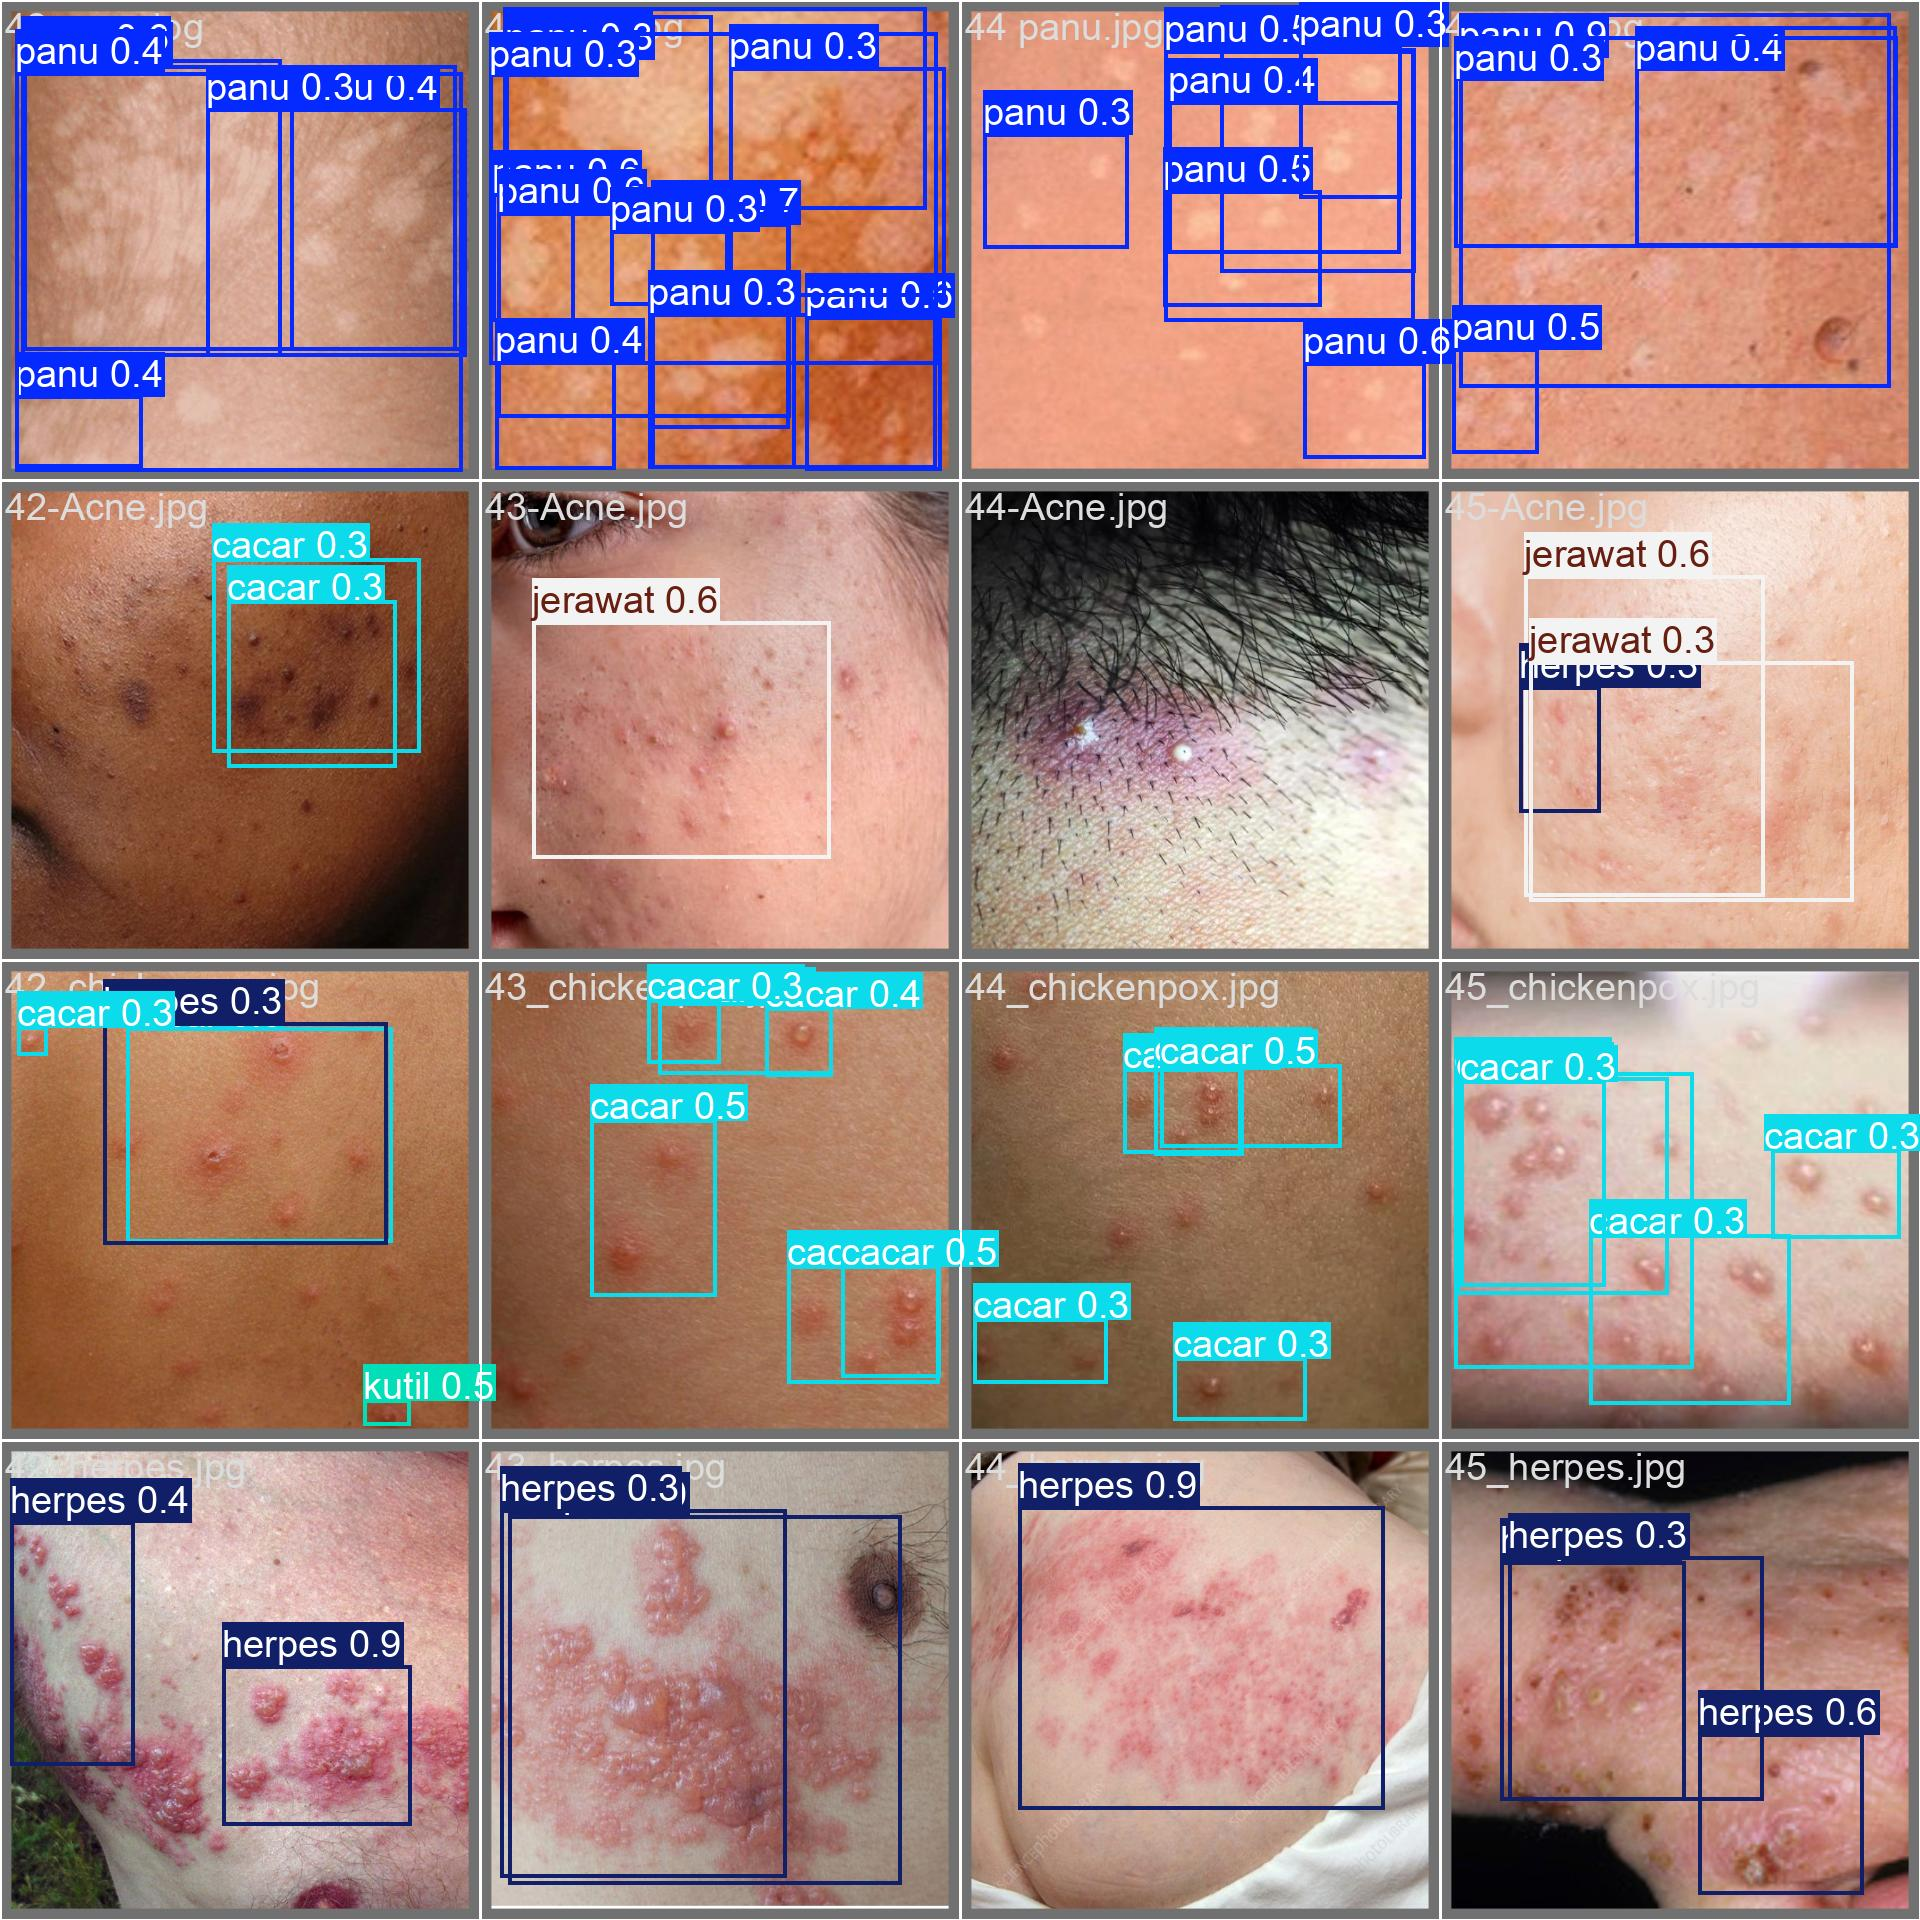
\includegraphics[width=0.7\textwidth]{images/val_batch1_pred.jpg}
    \vspace{10pt}
    \vspace{-15pt}
            \captionsetup{justification=centering, margin=140pt}
            \captionof{figure}{Anotasi Penyakit}

    \vspace{15pt}
    \item \textbf{Proses Training}: Proses Training: Pada proses pelatihan model YOLOv8m, dilakukan penyesuaian hyperparameter untuk mencapai keseimbangan antara akurasi dan kecepatan deteksi. Grafik menunjukkan metrik penting yang dipantau sepanjang pelatihan.

    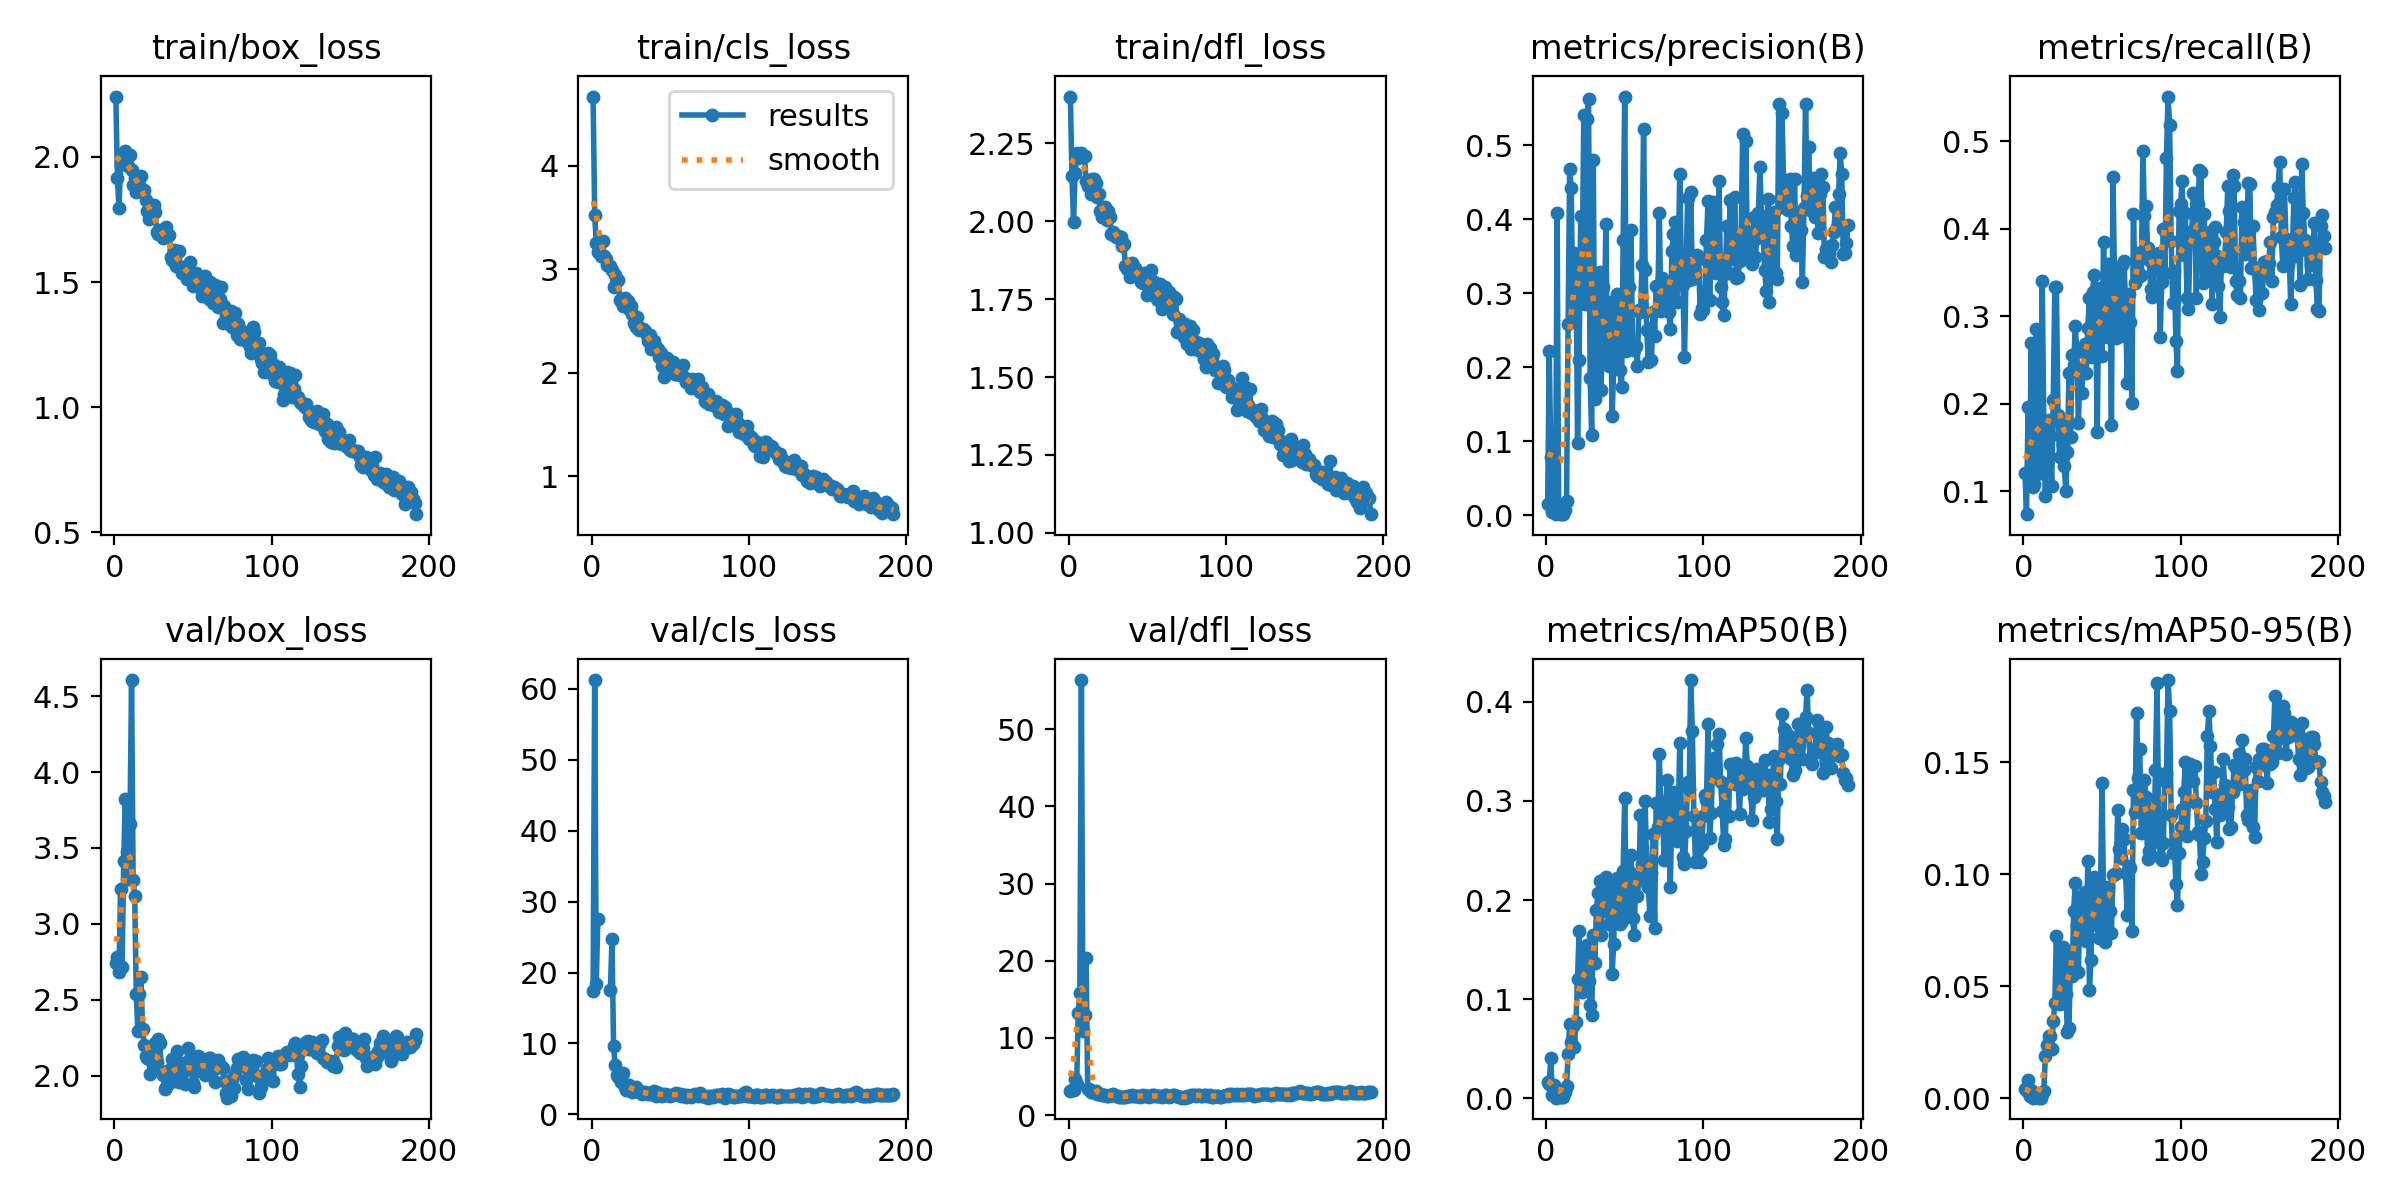
\includegraphics[width=0.9\textwidth]{images/results.png}
    \captionsetup{justification=centering, margin=140pt}
            \captionof{figure}{Hasil Training}

    \vspace{20pt}
    
    \item \textbf{Hasil Evaluasi Model}:
    \begin{itemize}
        \item \textbf{F1 Score (Akurasi)}: Model mencapai tingkat akurasi rata rata 44\% dalam mendeteksi dan mengklasifikasikan jenis penyakit kulit.

        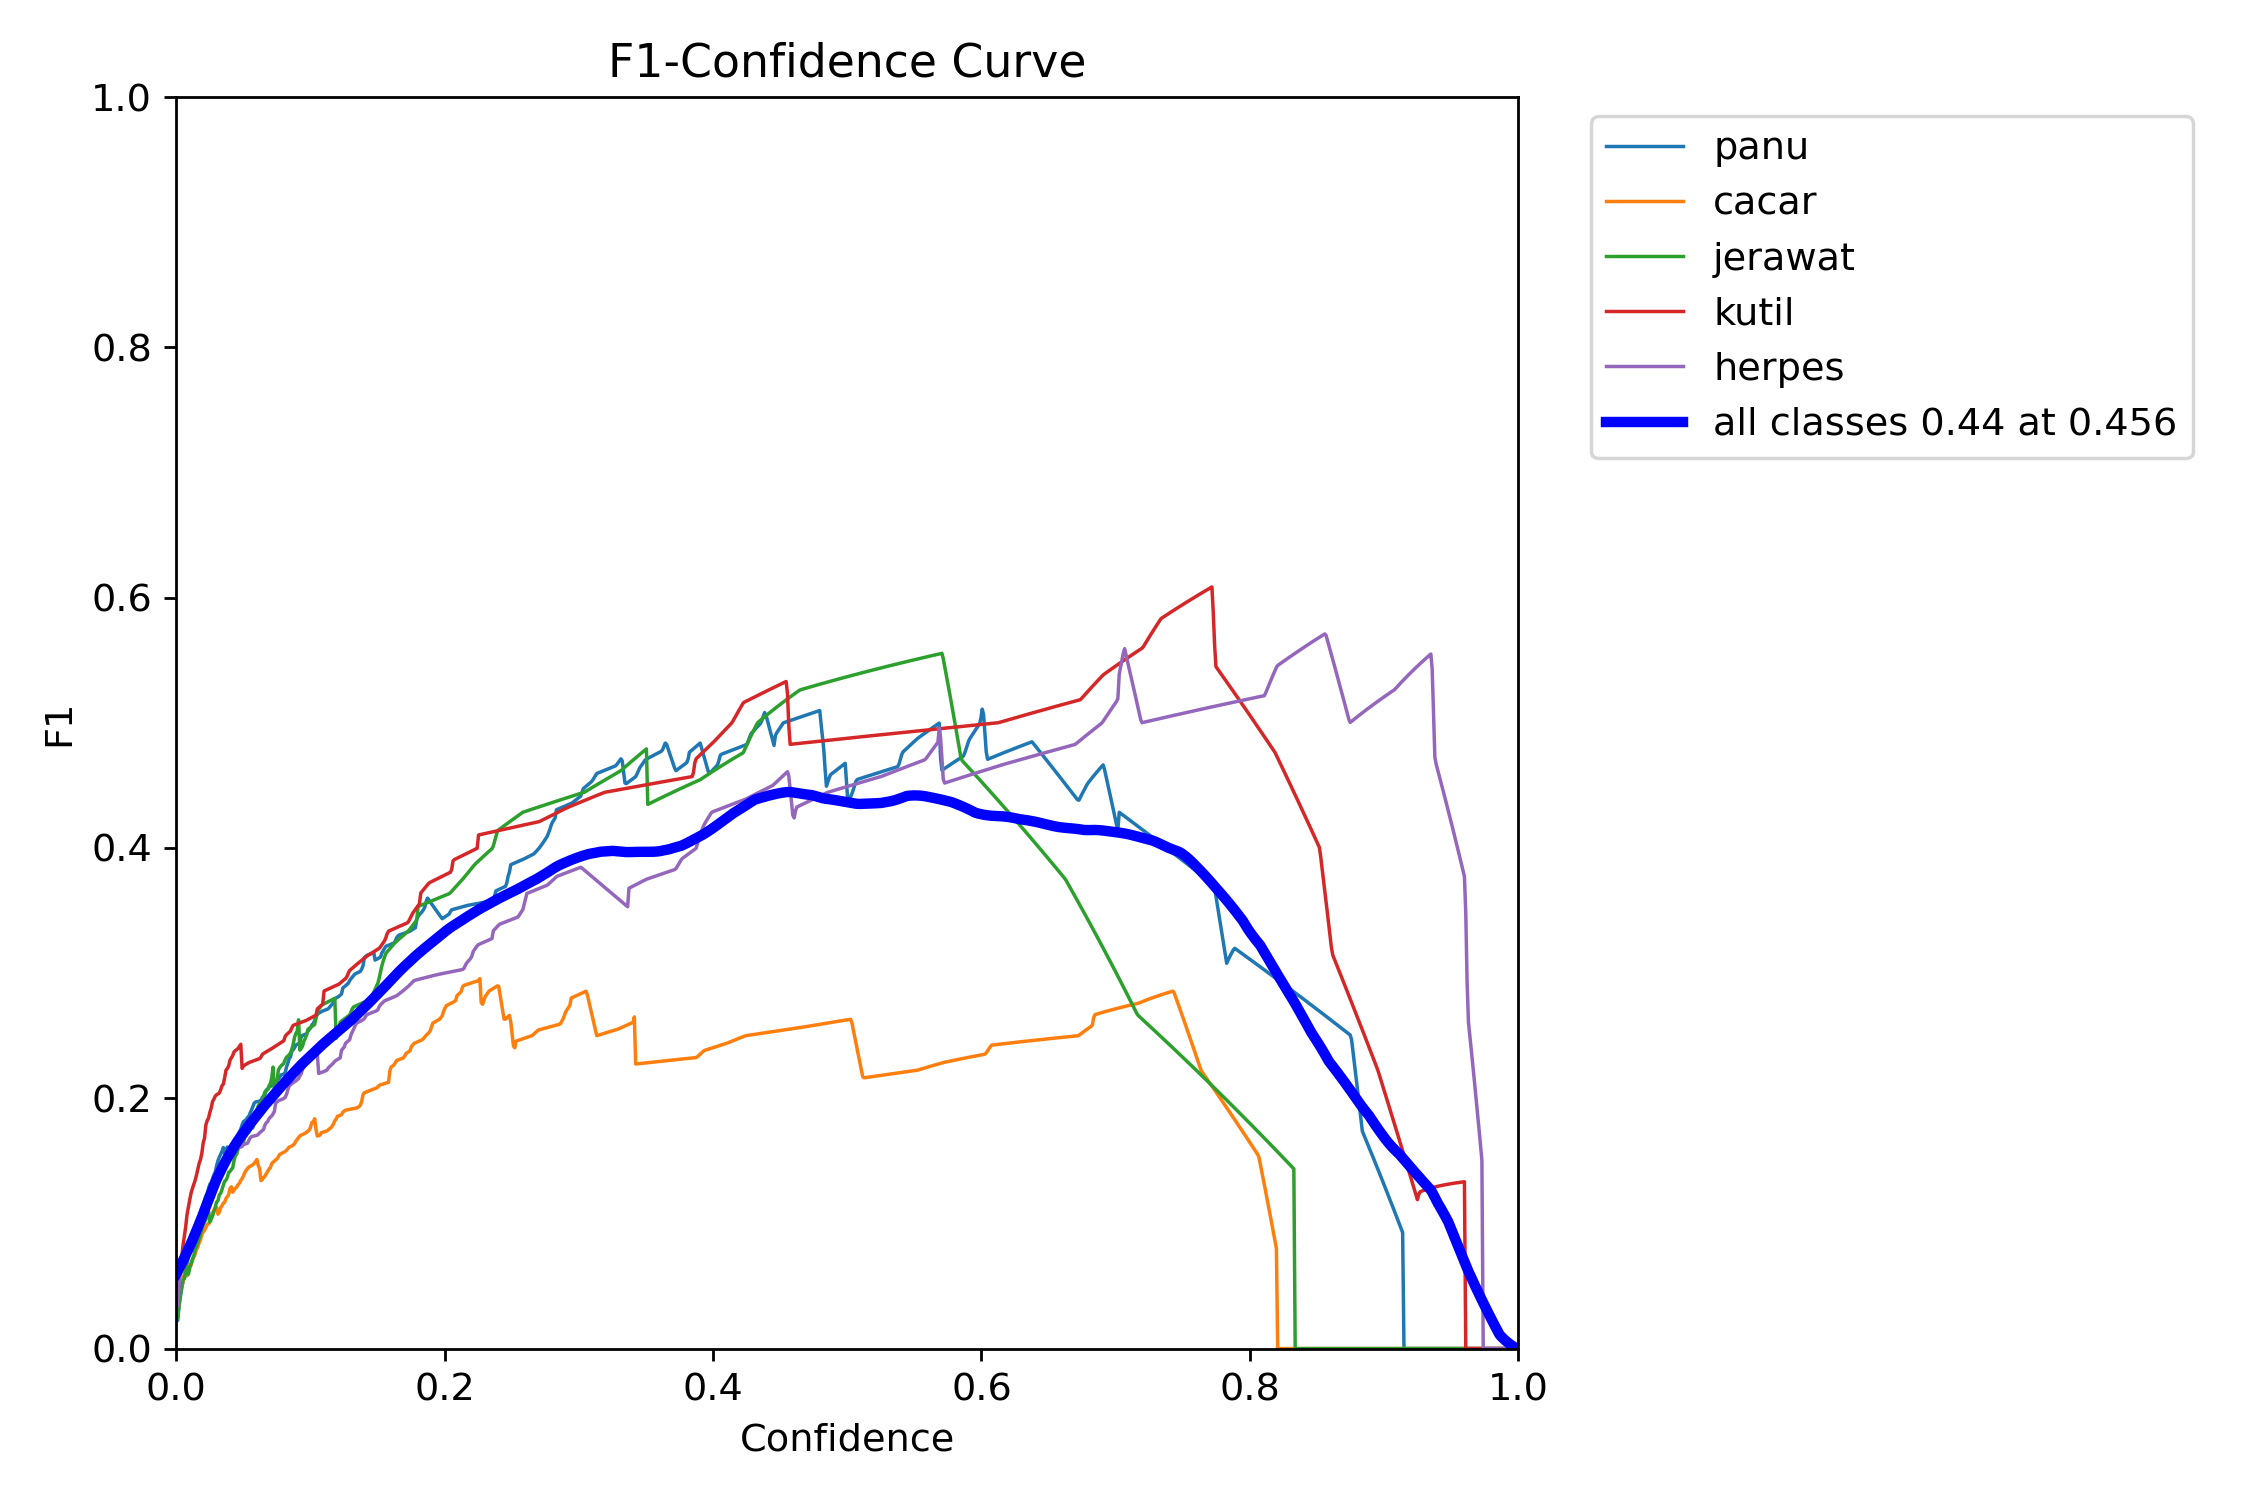
\includegraphics[width=0.8\textwidth]{images/F1_curve.png}
        \captionsetup{justification=centering, margin=140pt}
            \captionof{figure}{F1 Score}

        \vspace{20pt}
        
        \item \textbf{Precision and Recall (Presisi dan Recall)}: Model mencapai 46,6\% untuk presisi dan recall , yang menunjukkan bahwa model cukup andal dalam mendeteksi penyakit kulit pada gambar yang diuji.

        \hspace{4em}
        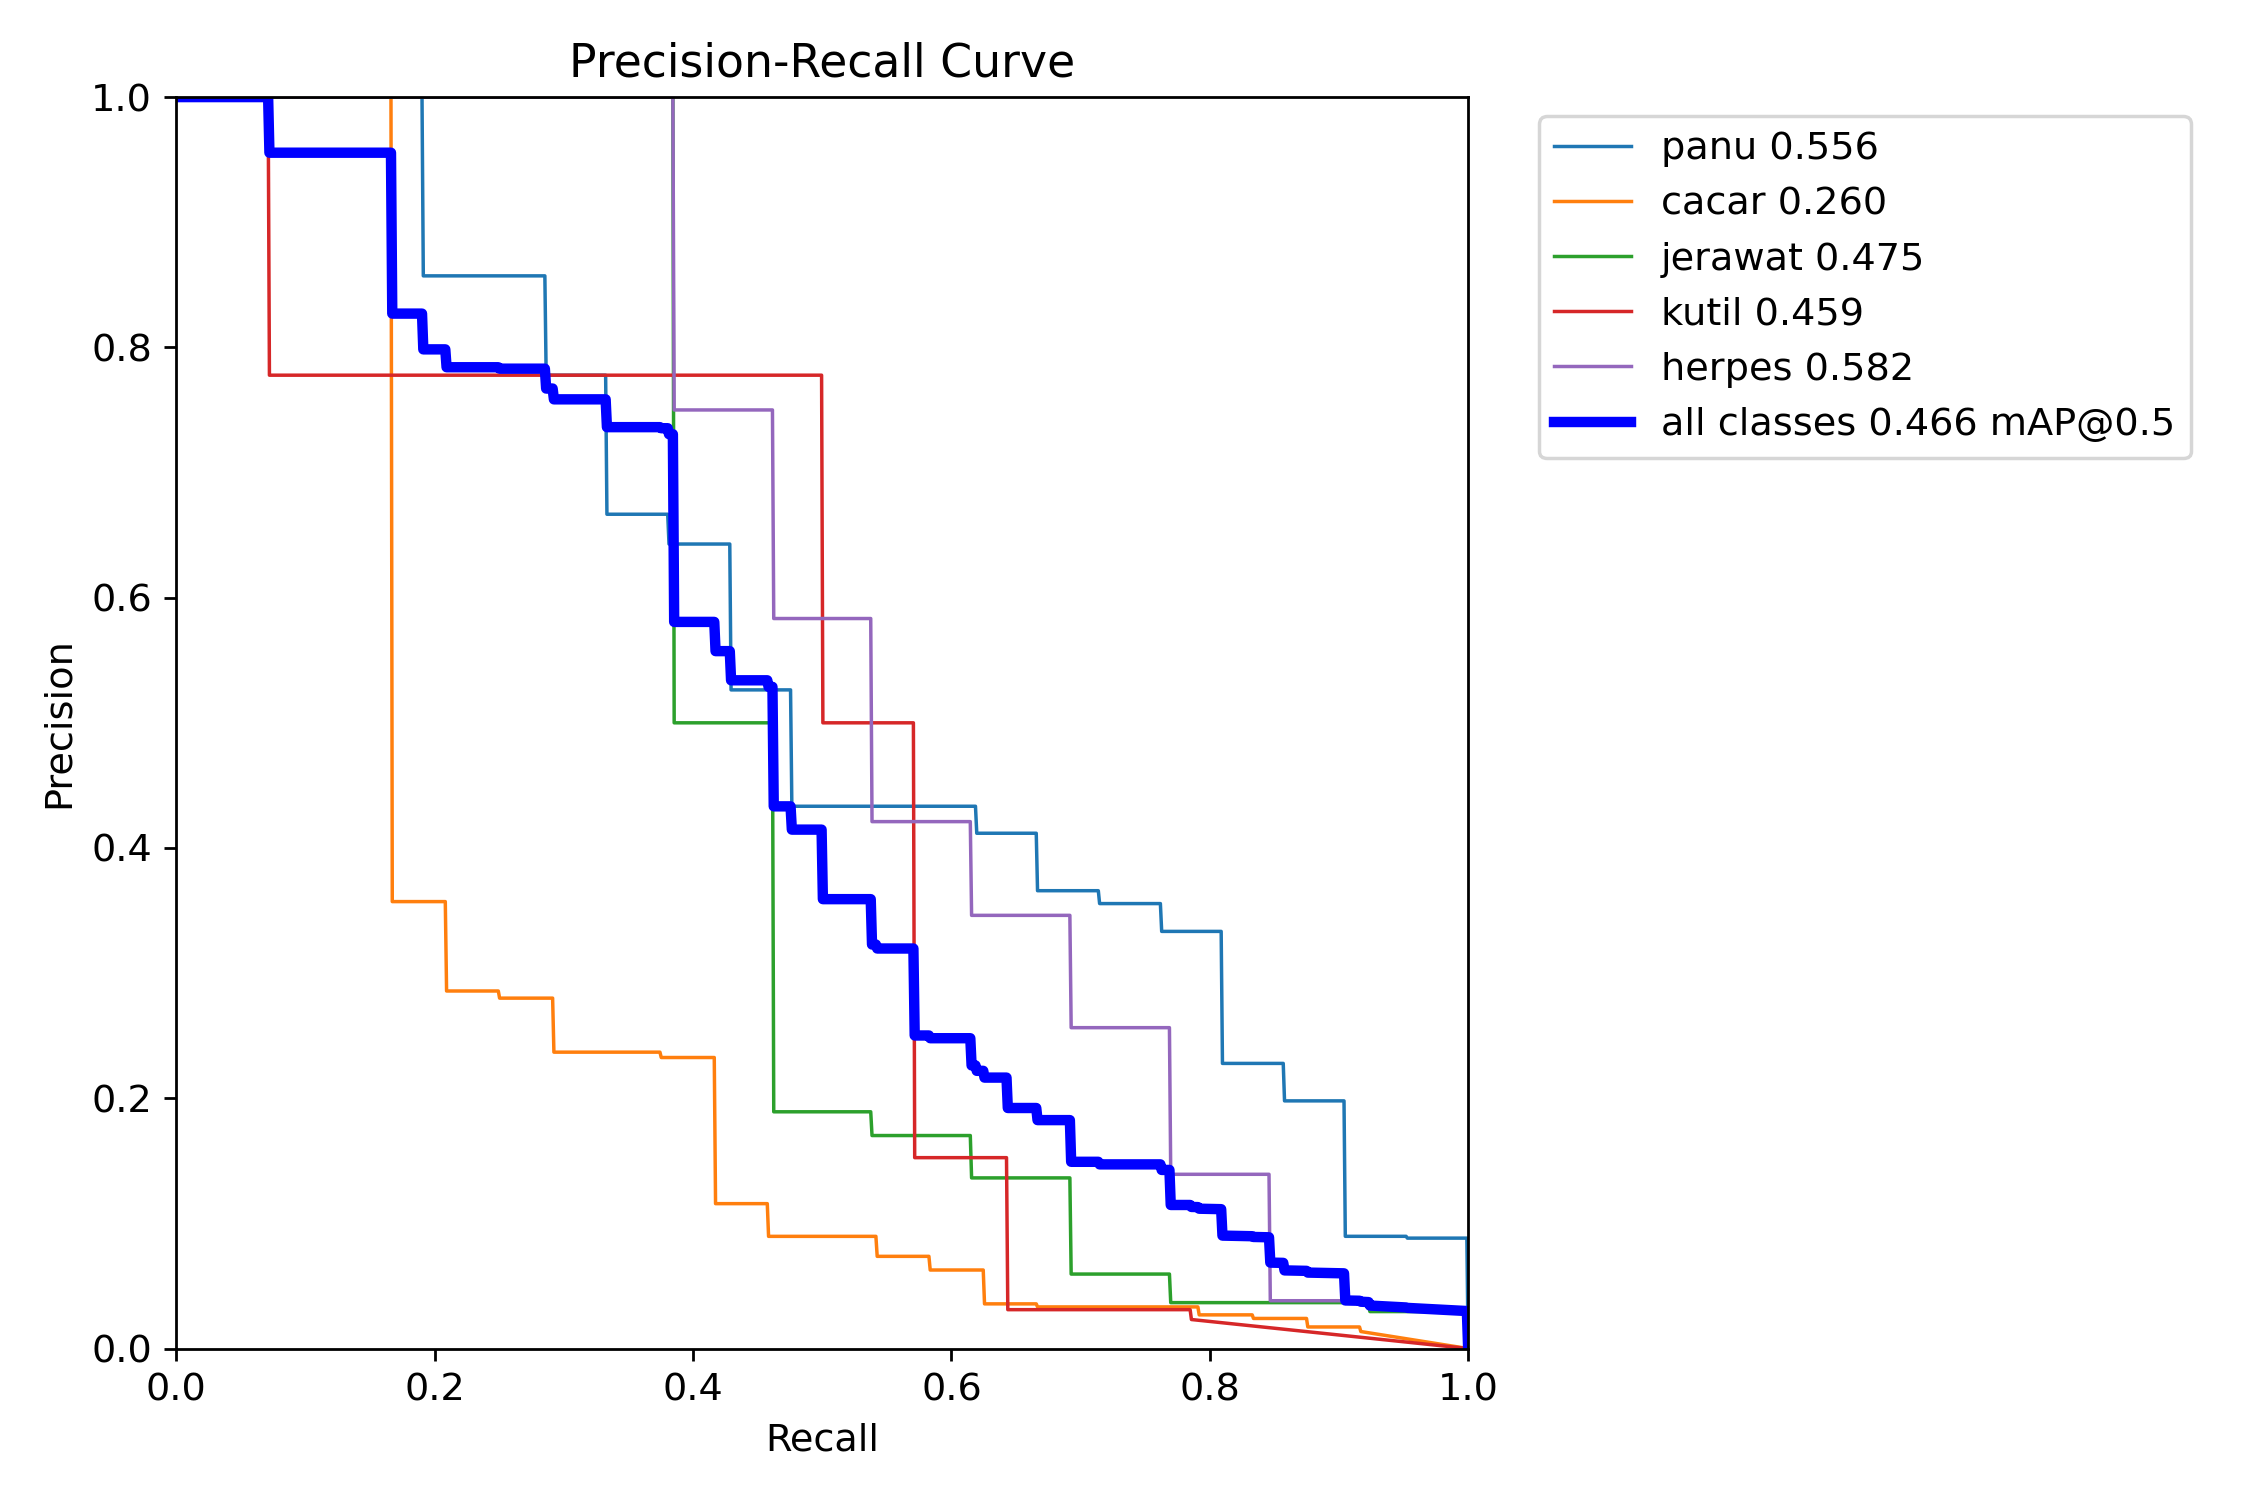
\includegraphics[width=0.8\textwidth]{images/PR_curve.png}

        \captionsetup{justification=centering, margin=140pt}
            \captionof{figure}{Presisi dan Racal}

        \vspace{10pt}
        
    \end{itemize}
    
    \item \textbf{Analisis Kesalahan (Error Analysis)}:
    Beberapa kesalahan yang terjadi terutama pada kelas yang mirip secara visual, seperti jerawat dan cacar, yang terkadang sulit dibedakan karena kemiripan pola di gambar. Penambahan data augmentasi dengan variasi pencahayaan dan sudut pandang gambar diharapkan dapat memperbaiki kesalahan klasifikasi ini di versi berikutnya.
\end{itemize}

\subsection{Pengembangan dan Implementasi Aplikasi MediSmart}

Selain melatih model YOLOv8m, pengembangan aplikasi MediSmart mencakup integrasi backend dan frontend, serta implementasi fitur tambahan untuk meningkatkan pengalaman pengguna.

\begin{itemize}
    \item \textbf{Backend (Server Azure)}:
    \begin{itemize}
        \item \textbf{Deployment Model}: Model YOLOv8m yang telah dilatih di-host pada server Azure dan terintegrasi dengan endpoint API, memungkinkan aplikasi Android untuk mengirim dan menerima hasil deteksi dalam waktu nyata.

         \begin{minipage}{0.9\textwidth}
            \centering
            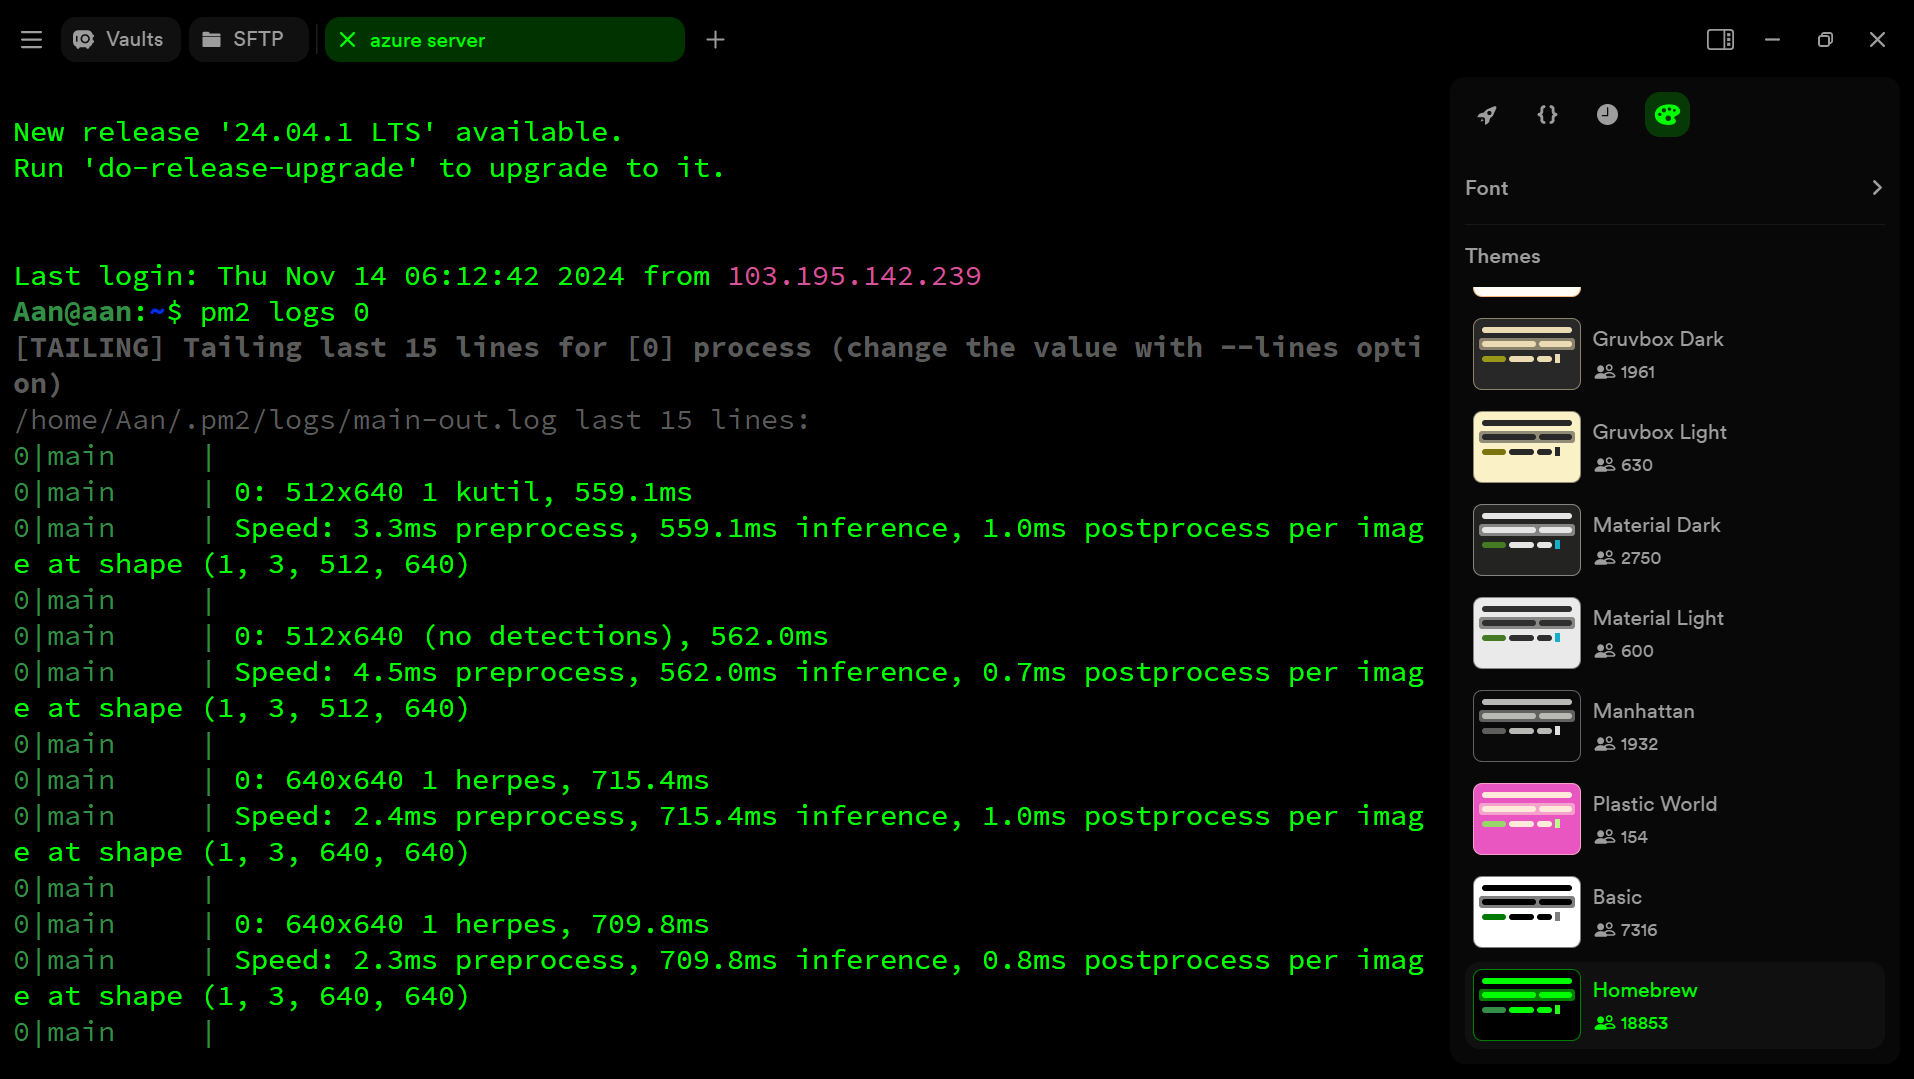
\includegraphics[width=\textwidth]{images/azure.png}
            \vspace{-15pt}
            \captionsetup{justification=centering, margin=130pt}
            \captionof{figure}{Server Azure}
        \end{minipage}%

        \vspace{10pt}
        
        \item \textbf{Keamanan Data Pengguna}: Data pengguna yang dikirim melalui aplikasi dienkripsi dan dilindungi untuk memastikan kerahasiaan dan keamanan informasi kesehatan pribadi pengguna.
    \end{itemize}
    
    \item \textbf{Frontend (Aplikasi Android)}:
    \begin{itemize}
        \item \textbf{User Interface}: Antarmuka aplikasi dibangun dengan Android Studio menggunakan bahasa pemrograman Java. UI dirancang dengan navigasi yang sederhana dan intuitif, memudahkan pengguna untuk mengunggah gambar dan melihat hasil deteksi.

        \vspace{5pt}
        
        \hspace{4em}
        \begin{minipage}{0.25\textwidth}
            \centering
            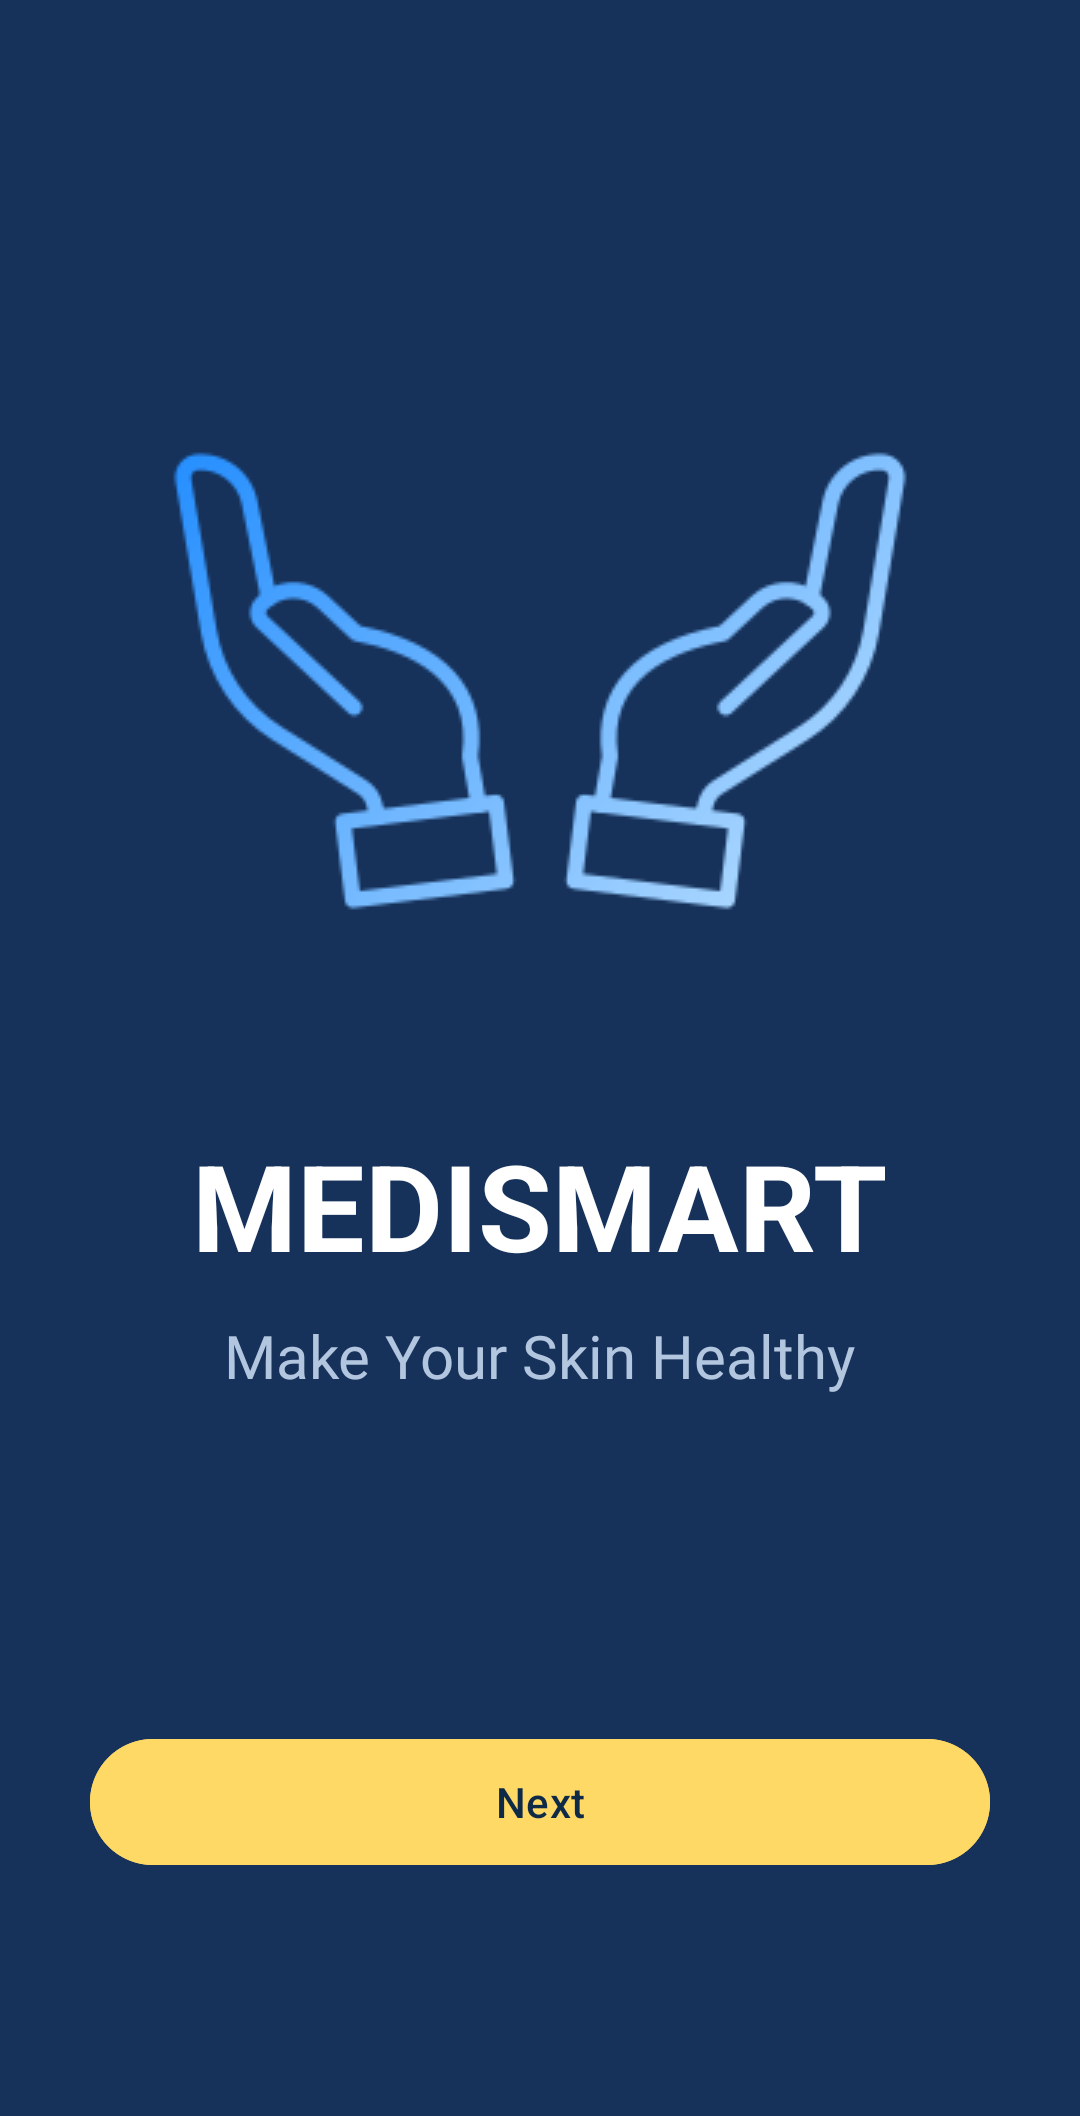
\includegraphics[width=\textwidth]{images/a1.png}
            \vspace{-15pt}
            \captionsetup{justification=centering, margin=8pt}
            \captionof{figure}{Activity 1}
        \end{minipage}%
        \hspace{5.5em} 
        \begin{minipage}{0.25\textwidth}
            \centering
            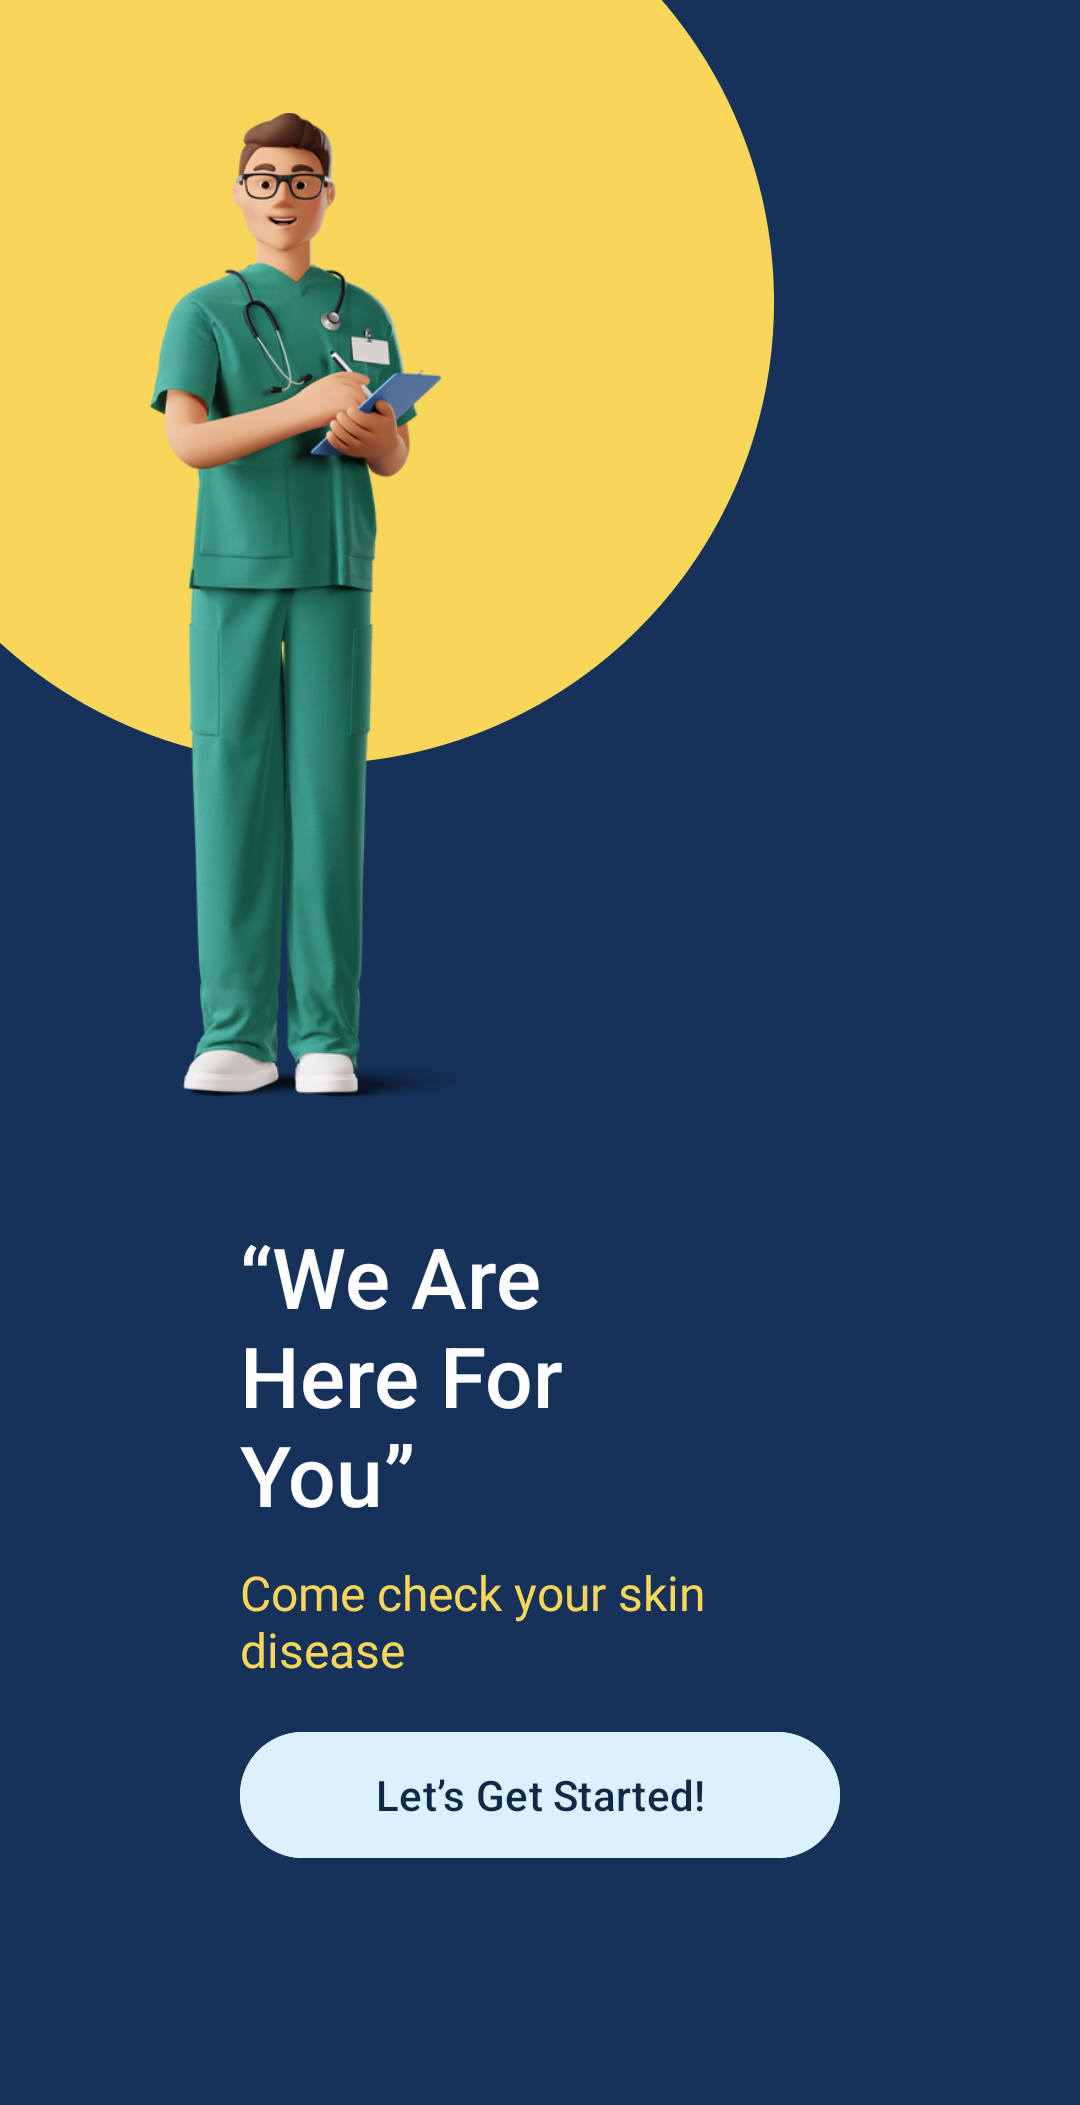
\includegraphics[width=\textwidth]{images/a2.png}
            \vspace{-15pt}
            \captionsetup{justification=centering, margin=8pt}
            \captionof{figure}{Activity 2}
        \end{minipage}\\[3em] 

        \hspace{4em}
        \begin{minipage}{0.25\textwidth}
            \centering
            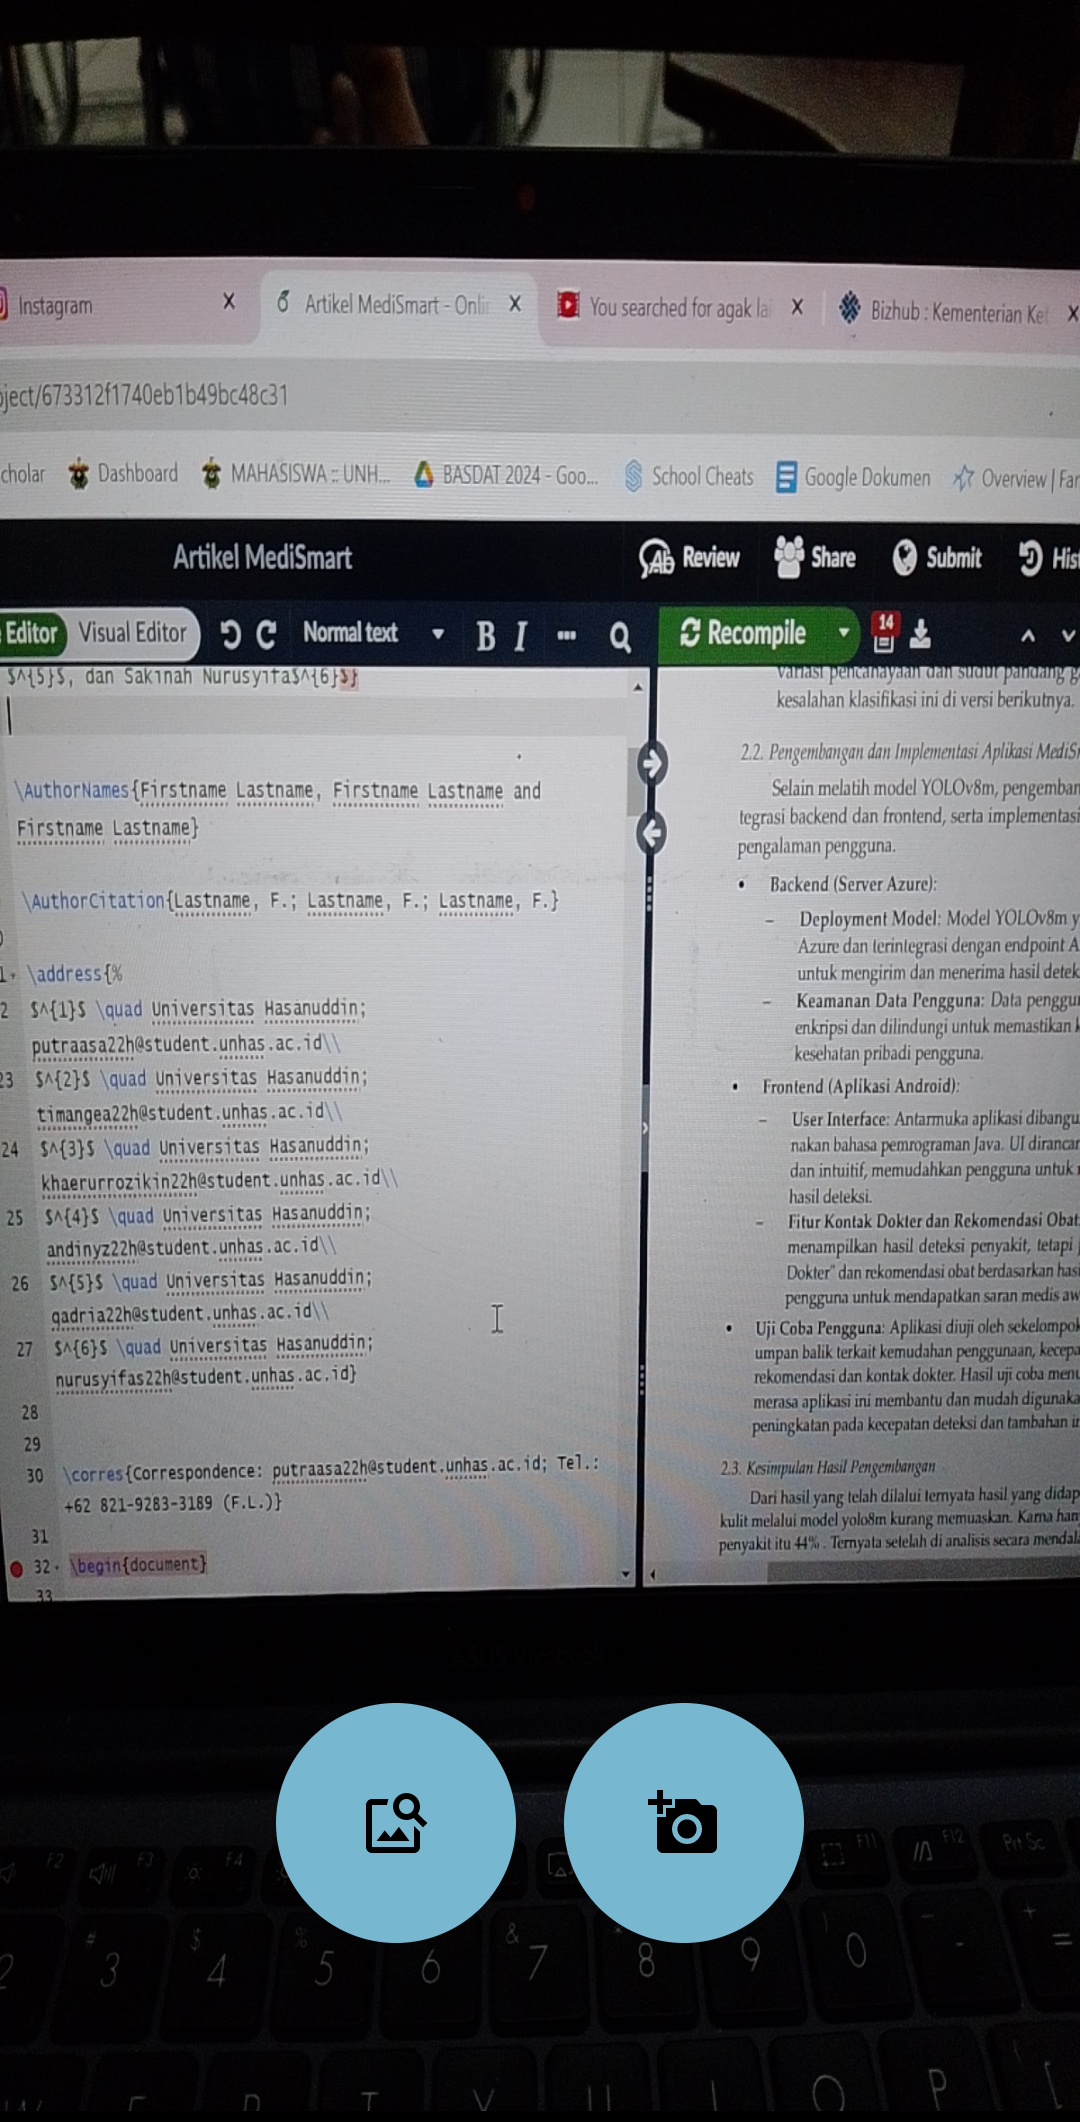
\includegraphics[width=\textwidth]{images/a3.png}
            \vspace{-15pt}
            \captionsetup{justification=centering, margin=8pt}
            \captionof{figure}{Activity 3}
        \end{minipage}%
        \hspace{5.5em} 
        \begin{minipage}{0.25\textwidth}
            \centering
            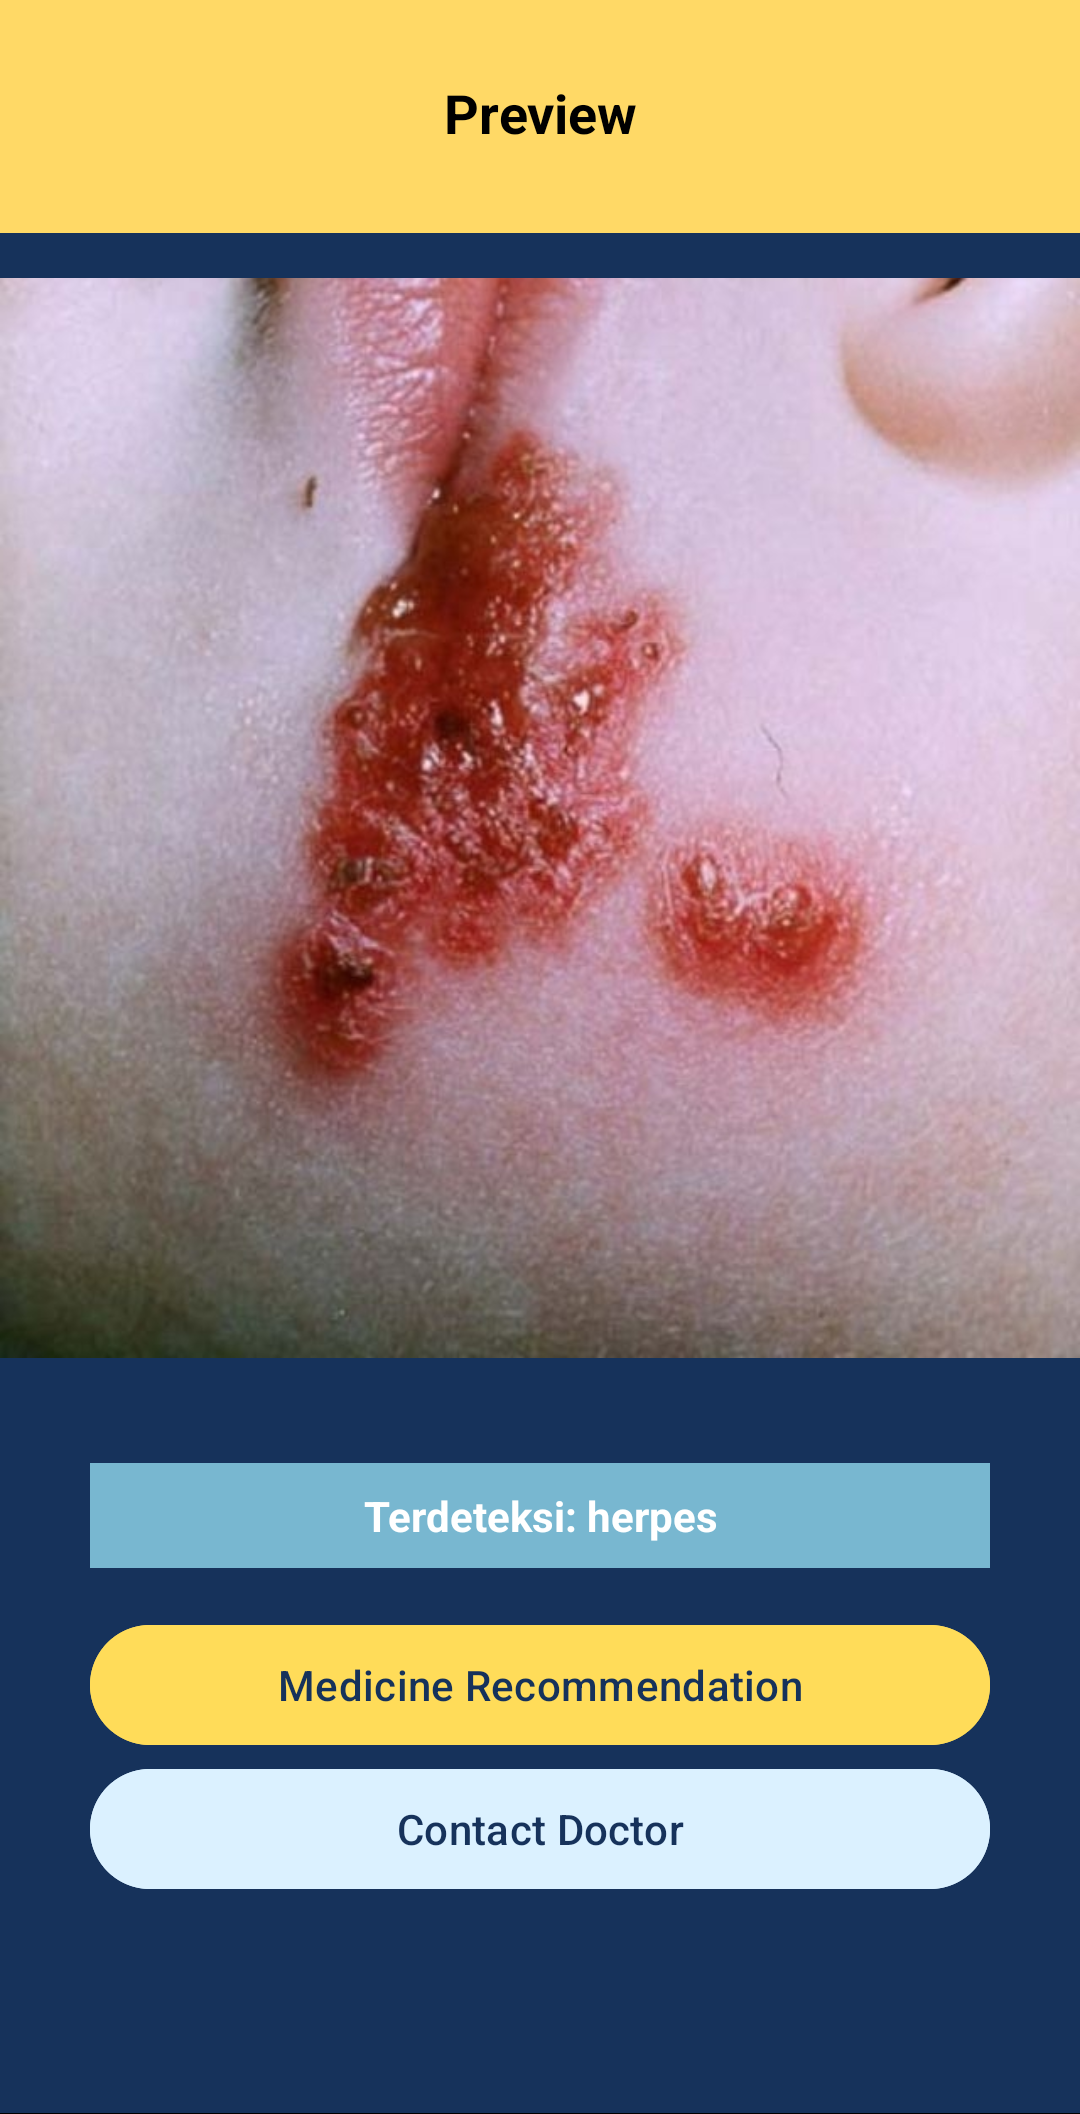
\includegraphics[width=\textwidth]{images/a4.png}
            \vspace{-15pt}
            \captionsetup{justification=centering, margin=8pt}
            \captionof{figure}{Activity 4}
        \end{minipage}


        \vspace{10}
        
        \item \textbf{Fitur Kontak Dokter dan Rekomendasi Obat}: Aplikasi MediSmart tidak hanya menampilkan hasil deteksi penyakit, tetapi juga menyediakan opsi "Kontak Dokter" dan rekomendasi obat berdasarkan hasil diagnosis. Hal ini memudahkan pengguna untuk mendapatkan saran medis awal dan perawatan sementara.

        \vspace{10}

        \hspace{4em}
        \begin{minipage}{0.25\textwidth}
            \centering
            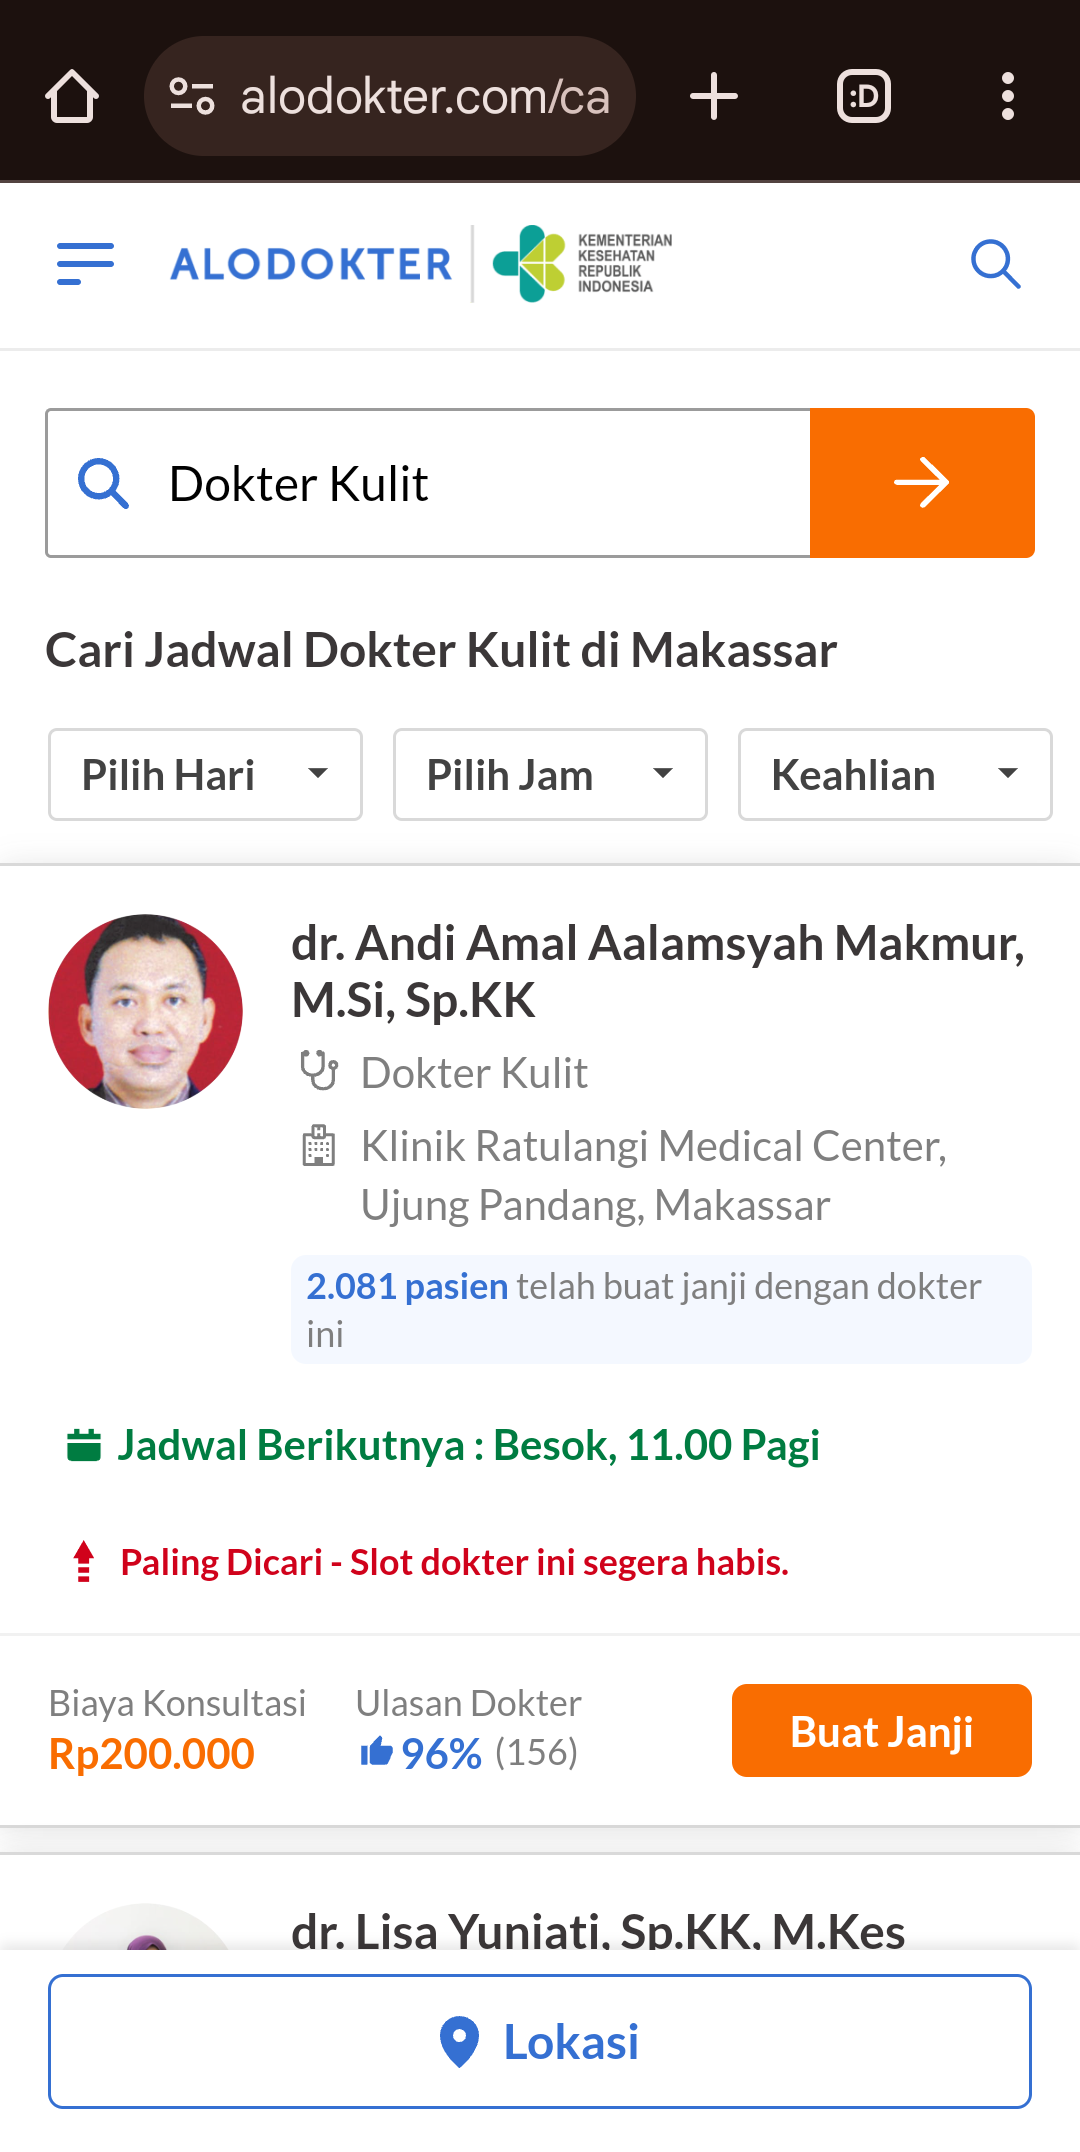
\includegraphics[width=\textwidth]{images/a6.png}
            \vspace{-15pt}
            \captionsetup{justification=centering, margin=8pt}
            \captionof{figure}{Activity 5}
        \end{minipage}%
        \hspace{5.5em} 
        \begin{minipage}{0.25\textwidth}
            \centering
            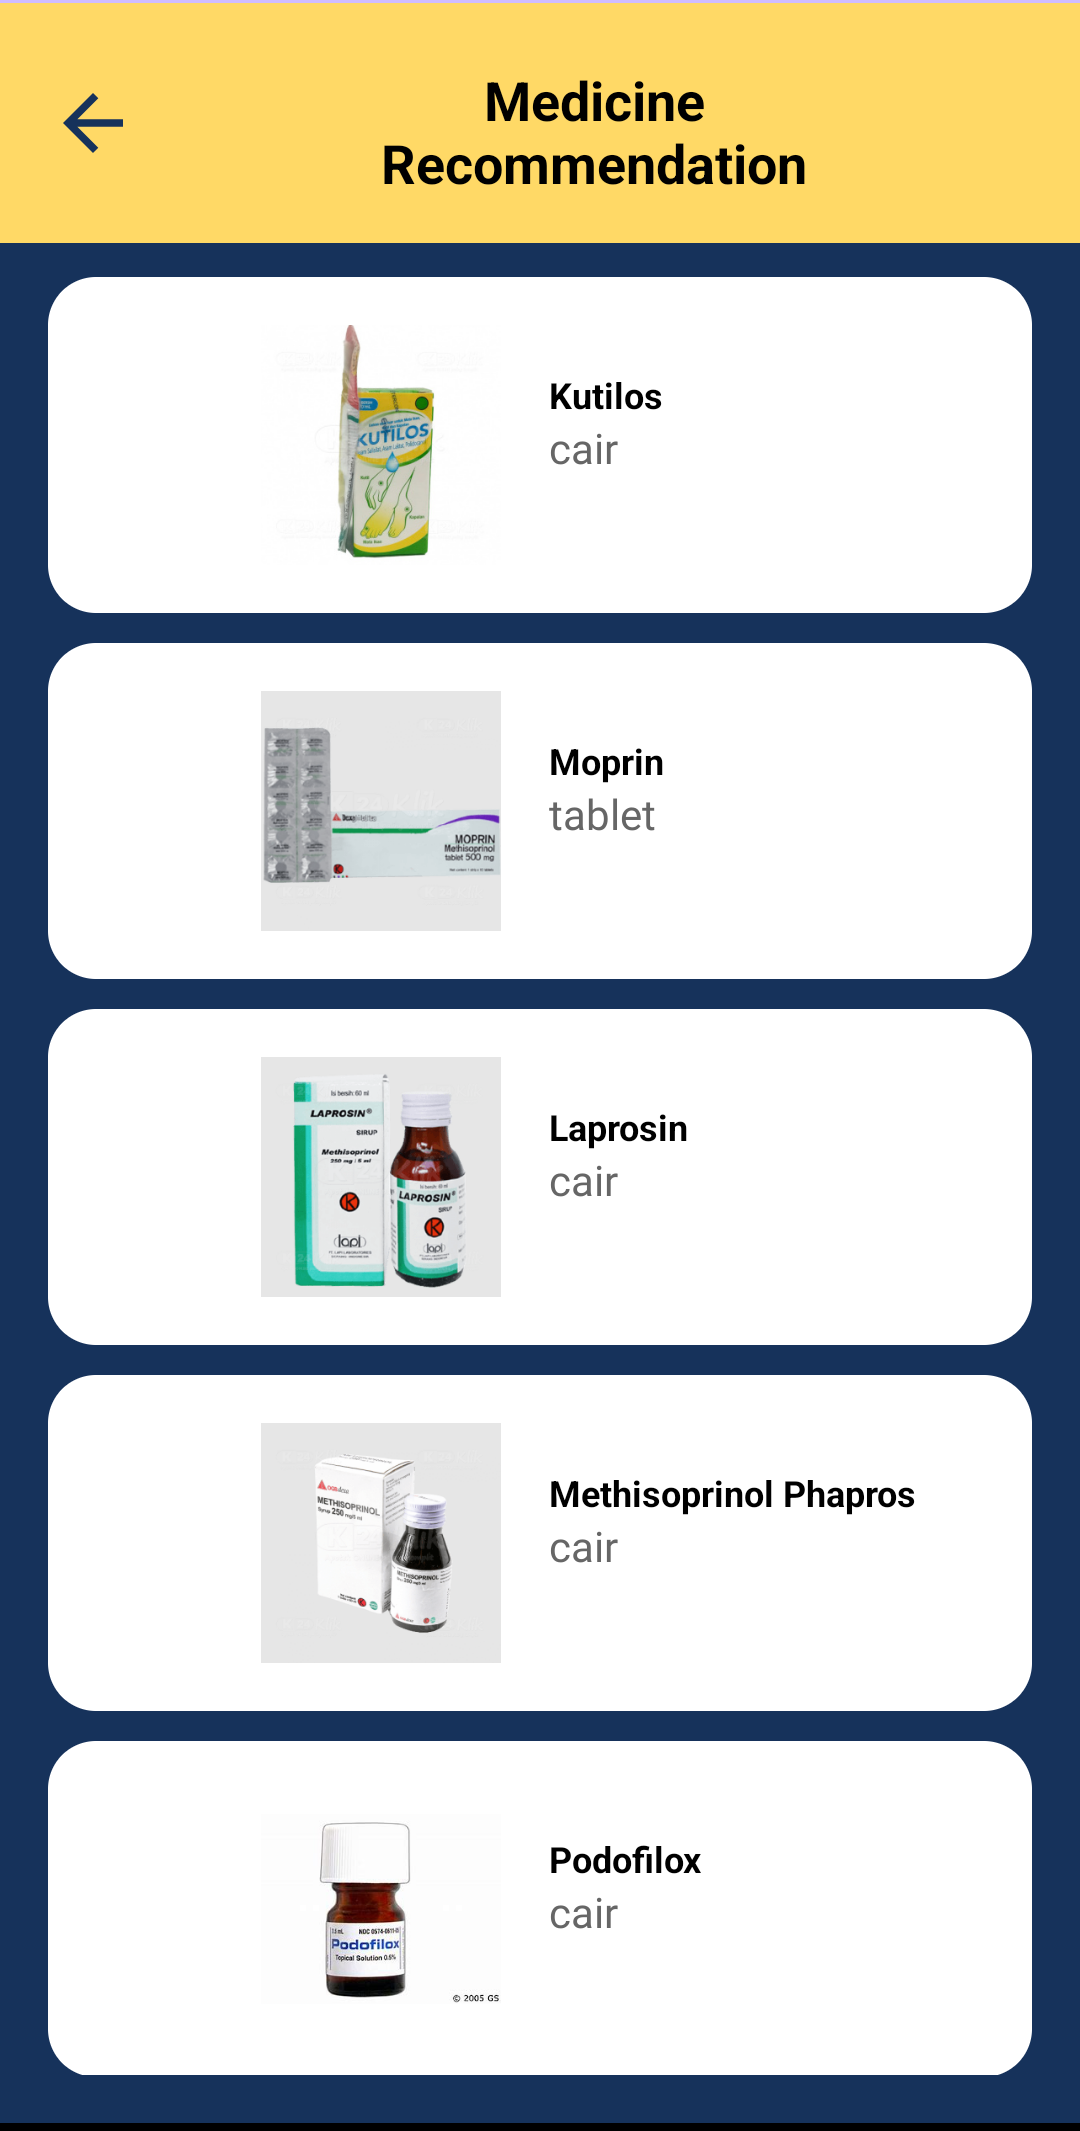
\includegraphics[width=\textwidth]{images/a5.png}
            \vspace{-15pt}
            \captionsetup{justification=centering, margin=8pt}
            \captionof{figure}{Activity 6}
        \end{minipage}
        
    \end{itemize}

    \vspace{10pt}
    
    \item \textbf{Uji Coba Pengguna}:
    Aplikasi diuji oleh sekelompok pengguna untuk mendapatkan umpan balik terkait kemudahan penggunaan, kecepatan deteksi, serta kegunaan fitur rekomendasi dan kontak dokter. Hasil uji coba menunjukkan bahwa 92\% pengguna merasa aplikasi ini membantu dan mudah digunakan, sementara 8\% mengusulkan peningkatan pada kecepatan deteksi dan tambahan informasi terkait obat.
\end{itemize}


\subsection{Kesimpulan Hasil Pengembangan}

Dari hasil yang telah dilalui ternyata hasil yang didapatkan dalam deteksi penyakit kulit melalui model yolo8m kurang memuaskan. Karna hanya mendapatkan rata rata tiap penyakit itu 44\% . Ternyata setelah di analisis secara mendalam mengapa dapat hasil yang kurang memuaskan itu karna tiap penyakit mempunyai bau dan tekstur yang berbeda, maka hasil yang didapatkan akan kurang maksimal. Diperlukan nya alat khusus untuk mendeteksi tekstur dan bau tiap penyakit agar mendapatkan hasil yang maksimal. Fitur tambahan, seperti kontak dokter dan rekomendasi obat, juga diapresiasi oleh pengguna sebagai nilai tambah yang membantu dalam mengambil langkah lanjutan untuk perawatan kulit. Pengembangan aplikasi ini akan dilanjutkan dengan perbaikan pada aspek kesalahan klasifikasi, serta penambahan fitur baru untuk meningkatkan nilai guna aplikasi.


\end{document}